\chapter{\label{ch:lit_review} Literature Review}

Integrating quantum computers to current classical systems has proven to be a difficult endeavour because of the differences between classical bits and qubits. Properties of qubits such as superposition and entanglement also make it difficult to construct heterogeneous computing systems consisting of quantum processing units (QPUs), classical central processing units (CPUs), and graphical processing units (GPUs). This chapter presents a review of existing literature on modelling quantum computer architecture on a classical machine. 

The review focuses on previous implementations and simulations of interfaces between quantum and classical computers in a heterogeneous computing system - in alignment with the scope of this paper. Furthermore, guidelines for conducting accurate FPGA-based quantum computer emulations are discussed with respect to quantum algorithm implementation and communicating the output from a quantum computer as bits to a classical computer. From this context, previous literature is use to expand the knowledge of quantum computing through an investigation of bit encoding methodologies, quantum algorithm and quantum circuit implementations in engineering applications, qubit decoding, as well as different types of quantum computer architectures that exist. In particular, the scope of the paper is limited to quantum computing algorithms that can be emulated using reconfigurable Programmable Logic Devices (PLDs) such as the FPGA.  As such, this overview of the literature accumulates quantum gate simulations that can be implemented directly at the physical level with both trapped ions and superconducting circuits.

The chapter begins by discussing applications of quantum circuit theory and implementations in quantum computing algorithms that can be performed on a FPGA-based emulated quantum computer. Then, the study investigates quantum computing architectures, communication protocols and interfaces for transmitting data between classical and quantum computers. In particular, the use of data encoding methods that have been previously implemented in engineering are discussed. The review terminates with a discourse into the overall integration and accurate simulation of heterogeneous systems containing QPUs. 

\section{Quantum Computer Realisation Criteria}


Emulating a quantum computing system on a classical device such as an FPGA requires an understanding of the fabrication of qubits, their quantum mechanical properties, and contraints on the operations that can act on them. To successfully model a quantum computer using the classical bits, it suffices to investigate the physical realisation and behaviour of qubits. In the year 2000, DiVincenzo detailed five criterion for realising a quantum computer, starting with a physical system containing a collection of qubits \cite{divincenzo2000physical}. Qubits have been realised physically as photons, nitrogen vacancies in diamonds or quantum dots in solid state systems \cite{marinescu2005promise}. Electron spin and its phase have also been controlled and manipulated to establish quantum gate transformations. In all cases, the qubits must be \textit{well-characterised}, as described in DiVincenzo's first criterion for quantum computers \cite{divincenzo2000physical}. In other words, qubits must satisfy the requirement that the general state must be expressed as a vector space with eigenvectors, $\ket{0}$ and $\ket{1}$, and normalised amplitudes, $\alpha$ and $\beta$, as shown in equation \ref{eqn:qstate}. Consequently, mappings between classical bits to qubits cannot be injective because of this fundamental difference between the two representations of units of information. However, FPGAs provide high fidelity for modelling quantum computers through logic blocks that can be connected in networks of arbitrary depth \cite{wolf2004fpga}. Since one of the objectives of this paper is to map the physical behaviour and interactions of qubits in quantum computing systems to the \gls{personality} (or program) of an FPGA that is interwoven into its logic structure.

\subsection{Well-Characterised Qubits for Realising a Quantum Computer}

According to DiVincenzo, the normalised coefficients should be accurately known. DiVincenzo extended the term "well-characterised" to mean several different things, including the presence of couplings to and interactions with other states of the qubit as implemented by Bluhm et al. who also considered the couplings of qubits to external fields by \gls{hyperfine structure}s \cite{divincenzo2000physical, bluhm2011dephasing}. DiVincenzo extends this application to two-qubit systems to emphasise that the general state of such a quantum computer can be expressed as a four-dimensional vector that can be separated into one-dimensional distinguishable sub-states of two systems \cite{divincenzo2000physical}. Using this example, DiVincenzo also cautions against the common error of considering a single-qubit system in superposition as a two-qubit system \cite{divincenzo2000physical}. Rather, such single-qubit systems that can be in two states simultaneously, must be considered as a vector space that is spanned by the states $\ket{01}$ and $\ket{10}$ \cite{divincenzo2000physical}. In modelling a quantum computer on a FPGA, the multi-level \gls{fine-grained} combinational logic elements and connectivity networks in the fabric of the device can be leveraged to emulate qubit superposition and qubit couplings in the computational basis. 

Kimble et al. implemented a method that uses a single quantum particle to describe a well-characterised qubit using measurements of the \gls{birefringence} of a single atom strongly coupled to a \gls{high-finesse} optical resonator (or cavity) ]\cite{turchette1995measurement}. Specifically, Kimble et al. demonstrated the conditional dynamics that are necessary for implementing quantum logic at the single-photon level between two frequency-distinct fields in an optical resonator by rotating the linear polarisation of a transmitted probe beam \cite{turchette1995measurement}. The well-characterised qubit was achieved from the nonlinear optical response of a Caesium (Cs) atom coupled to a cavity field with a cavity length of $\SI{56}{\micro\meter}$ \cite{turchette1995measurement}. Interactions between the photons inside the atom cavity device were investigated using the transmission of monochromatic coherent-state pump and probe beams, which were independently tunable in frequency, power and polarisation \cite{turchette1995measurement}. To quantify the strength of the photon-photon interactions, the pump and probe input fields in the quantum experiment were prepared as uncorrelated coherent states with small normalised amplitudes $|\alpha|^2$ and $|\beta|^2$ \cite{turchette1995measurement}.  Kimble et al. extended the prospects for quantum based logic by introducing the quantum phase gate (QPG) and extracting the relevant phase shifts for the truth table of the gate \cite{turchette1995measurement}. In this paper, the input to the digital system are classical bits that model the behaviour of ideal single-photon qubits. The methodology considers the initialisation of the classical bits as well-characterised qubits on a logical level, and sets constraints on the behaviour of the logic elements and connections in the FPGA to resemble the nature of the physically realised qubits. To model the preparation of uncorrelated coherent states in the emulation, qubits can be represented as a vector of size $2^n$ with complex amplitudes. Other properties of qubits - such as the no-cloning property which prohibits the duplication of a quantum state - have to be taken account as they introduce constraints on the how information should be transferred through the FPGA-emulated quantum computer.

In a 2022 study on the control of qubit transmission between quantum systems, Li, Zhang and Wu described the term "flying qubit" as quantum bits carried by travelling quantum fields \cite{li2022control}. Li et al. introduced their study by highlighting that in quantum networks, the transfer of quantum information between distant nodes can be physically realised by fabricating and capturing photons that encode these flying qubits which can range from quantum dots to microwaves from superconducting atoms \cite{li2022control}. A quantum dot can be described as a small semiconductor device with a core shell that containing free electrons \cite{marinescu2005promise}. Li et al. reference Eisaman et al.'s invited review article on single-photon sources and detectors which expands on the how photonic qubits can be generated "on-demand" using quantum dots \cite{li2022control, eisaman2011invited}.  In their 2011 article, Eisaman et al. describe the use of semiconductor quantum dots to facilitate the radiative recombination of electron-hole pair which leads to single-photon emission \cite{eisaman2011invited}. The review adds that the small size of quantum dots results in a discrete energy structure for the electrons and holes. Furthermore, the radiative lifetime of single-photon emission from optically or electrically excited quantum dots, is in the order of $\SI{1}{\nano\second}$ or less \cite{eisaman2011invited}. In the case of optically induced single-photon emission in GaAs based semiconductor quantum dots, excitation is created by photon absorption that saturates the quantum system \cite{eisaman2011invited}. Hours et al. uses a similar approach by exciting a $\SI{100}{\micro\meter}$ diameter region on GaAs/GaAlAs quantum dot with a He-Ne laser  \cite{hours2003single}. All optical measurements presented by Hours et al. were performed at $\SI{10}{\kelvin}$ in order to form a stable ground state in the GaAs/GaAsAlAs quantum well \cite{hours2003single}. Therefore, it is important to note that unlike classical bits which can be represented as high or low voltages corresponding to 0 and 1, the fabrication of qubits as single-photon also requires detectors and considerations of metrics such as the radiative lifetime. In this paper, single-photon emission from optically or electrically excited quantum dots is emulated device clocks and the radiative lifetime is represented by the pulse width.

\subsection{The Ability To Initialised Qubits to A Fiducial State}

DiVincenzo's second criterion required for the implementation of quantum information systems is the ability to initialise the state of the qubits to a simple \gls{fiducial state} \cite{divincenzo2000physical}. DiVincenzo explains that this requirement arises from the elementary computing requirement that registers should be initialised to a known value before the start of a process \cite{divincenzo2000physical}. In addition, DiVincenzo elaborates that quantum error correction requires a continuous supply of qubits in a low-entropy state such as the $\ket{0}$ basis state \cite{divincenzo2000physical}. DiVincenzo cites the need for a continuous source of 0s rather than just an initial supply, as one of the challenges in proposed implementations of quantum computers \cite{divincenzo2000physical}. 

According to DiVincenzo, for physical systems, the two main approaches for initialising quantum qubits to a standard state include cooling the system when the ground state of its Hamiltonian is the first state, or to measure and project the system into the desired state or another state on which gate operations can be performed to achieve the desired state. Prior to the publication of DiVincenzo's criteria, Imamoglu et al. propose a quantum computer in which information could be stored in the two lowest electronic states of doped GaAs quantum dots \cite{sherwin1999quantum}. Imamoglu et al. used two of the four lowest electronic energy levels to denote the states $\ket{0}$ and $\ket{1}$ for storing quantum information \cite{sherwin1999quantum}. The third energy level was used as an auxiliary state for performing conditional rotations of the state vector of the qubit \cite{sherwin1999quantum}. The state of an electron in the GaAs quantum dot was coherently manipulated by modulating the transition energies between states $\ket{0}$ and $\ket{1}$ using applied voltages to control the spacing between the energy levels \cite{sherwin1999quantum}. In fact, Imamoglu et al. describe inputting initial data as one of the core requirements for a universal quantum computer which can be achieved by arbitrary on-bit rotations effected using oscillations induced by a laser field \cite{sherwin1999quantum}.

%Another criteria for implementing a universal quantum computer that is described in literature by Imamoglu et al. relates to the ability to effect a \texttt{CNOT} gate operation as an additional requirement to initialisation of a state\cite{sherwin1999quantum}.

\subsection{Requirement for Sufficiently Long Relevant Decoherence Times}

The third criterion for implementing a quantum computer, as described DiVincenzo, states that for gate operations to be implemented physically, qubits in a quantum computer must have sufficiently long relevant decoherence times that are longer than gate operation times \cite{divincenzo2000physical}. Arguably, the primary reason for the difficulty in fabricating qubits is accounted for by the decoherence of quantum systems due to interactions of qubits with the environment. In short, decoherence times characterise the dynamics of a qubit \cite{divincenzo2000physical}. For example, in their study of electron spin decoherence in an isolated GaAs quantum dot, Khaetskii et al. found that decoherence, induced by hyperfine interactions within atomic nuclei, led to non-uniform hyperfine coupling \cite{khaetskii2002electron}. Hyperfine interactions of nuclei result from the small energy perturbations due to internally generated electric and magnetic fields. These interactions lead to \textit{decoherence}, which Marinescu describes as the randomisation of the internal state of a quantum computer due to interactions with the environment \cite{marinescu2005promise}. A key result of the study by Khaetsii et al. is that spin decay or decoherence is accompanied by the generation of quantum correlations between the electron spin and the nuclear spins which is viewed as the generation of entangled states between the qubit and its environment \cite{khaetskii2002electron}. This phenomenon is described as \textit{quantum parallelism} in decoherence. Markidis further defines \textit{quantum parallelism} - resulting from the interference of quantum state wave functions \cite{markidis2024quantum}. 

Decoherence is a principal mechanism for the emergence of classical behaviour in quantum computing that can be harnessed to perform quantum information processing \cite{divincenzo2000physical}. Conversely, if the decoherence time of a qubit is too long, then the capabilities of the quantum computer may not exceed the performance of a classical computer \cite{divincenzo2000physical}. According to DiVincenzo, decoherence may depend on the depend on the form of the initial state that can be affected by other quantum states of the qubit and in which the state amplitudes can change as well \cite{divincenzo2000physical}. Overall, the decoherence time of qubits of a system must be sufficiently long so that bits can be readout at the end of a computation \cite{sherwin1999quantum}. In their study of single-photon emission from individual GaAs/GaAlAs quantum dots, Hours et al. employ an oscillatory driving field to produce Rabi oscillations of excitons with an ultrafast radiative relaxation time in the range of 40 ps to reduce the effect of decoherence by dephasing mechanisms such as electron-phonon scattering \cite{hours2003single}. Rabi oscillations of excitons refer to the periodic alternation of electron-hole pairs between two-energy levels corresponding to a single-qubit rotation in a single quantum dot \cite{hours2003single, stievater2001rabi}. In their study of high performance emulation of quantum circuits, H\"{a}ner et al. suggest that unlike quantum simulations which directly mimic the operations that a quantum computer performs, including the effects of classical and quantum noise, a quantum emulator is only required to return the same result as a perfect and noiseless quantum computer would \cite{haner2016high}. This paper considers that although some properties of qubits such as decoherence times can be simulated, they cannot be emulated directly using classical bits.

Both Hours et al., as well as Gammon et al., excited the quantum dot through pumped laser pulses at a repetition rate in the range of $\SI{76}{\mega\hertz}$ to $\SI{82}{\mega\hertz}$, corresponding to quantum dot excitonic transitions with a time resolution determined by the pulse width, $T_1$, in the range between $\SI{6}{\pico\second}$ and $\SI{40}{\pico\second}$ \cite{hours2003single, stievater2001rabi}. In general, the $T_1$ \textit{decoherence time} characterises the duration of the transition of a qubit from an eigenstate with a higher discrete energy, such as the state $\ket{1}$, to an eigenstate in a lower energy level, such as the $\ket{0}$ basis state. The \textit{dephasing} time, $T_2$, corresponds to the time in which a qubit that is in superposition of states gradually loses phase. Gammon et al. showed that dephasing can be limited by energy relaxation at $\SI{4}{\kelvin}$ to achieve a dephasing times of $T_2 = 2T_1$ \cite{hours2003single}. For electrons in GaAs quantum dots, Bluhm et al. found that coherence times of about $\SI{1}{\micro\second}$ can revealed using spin-echo measurements at magnetic fields below $\SI{100}{\milli\tesla}$ \cite{bluhm2011dephasing}. Bluhm et al. use a spin qubit consisting of two isolated electrons confined in a double quantum dot that was created by applying negative voltages to metallic gates that locally deplete an electron gas at $\SI{90}{\nano\meter}$ below the GaAs wafer surface \cite{bluhm2011dephasing}. Bluhm et al. induced hyperfine interactions in a GaAs quantum dot by subjecting the two electrons to an effective magnetic field produced by nuclear spins \cite{bluhm2011dephasing}. The resulting Hilbert space of the logical qubit was spanned by the spin-up and spin-down combined states that can be equivalently represented as the basis states $\ket{10}$ and $\ket{01}$ \cite{bluhm2011dephasing}. In a programmable all-optical scheme for different one-qubit system, Goswami, Mandal and Mukhopadhyay implemented qubits using phase and intensity encoding of light with the help of the electro-optic modulators supported by MATLAB simulations \cite{mandal2023implementation}.

\subsection{Physical Preparation of Entangled Qubit Pairs}

Bluhm et al. initialised the ground state of the quantum system as a spin singlet with both electrons located in the neighbourhood of a single dot \cite{bluhm2011dephasing}. The electrons were successfully separated onto two quantum dots by sweeping the difference between the electrostatic potentials in the two dots to negative values, thereby preparing the Bell state $\ket{s}$, given by
\begin{align}\label{eqn:s-}
	\ket{s_-}	& = \frac{1}{\sqrt{2}}\ket{10} - \frac{1}{\sqrt{2}}\ket{01}
\end{align}
Additionally, Bluhm et al. found that very large detunings of the electrostatic potential difference between the electrons as well as the difference between the $\hat{z}$-components of the hyperfine fields in the two dots leads to energy splitting between the basis states and causes precession between the singlet state $\ket{s_-}$ and the triplet state $\ket{s_+}$, given by
\begin{align}\label{eqn:s+}
	\ket{s_+} & = \frac{1}{\sqrt{2}}\ket{10} + \frac{1}{\sqrt{2}}\ket{01}
\end{align}
The fluctuations induced by this splitting of electrons on the double quantum dots lead to dephasing of the qubit which drives coherent oscillations between the basis states \cite{bluhm2011dephasing}. Using this technique, Bluhm et al. achieved dephasing times $T_2$ exceeding $\SI{200}{\micro\second}$, which is sufficiently long to satisfy DiVincenzo's criterion regarding decoherence times - allowing a possible $10^5-10^6$ operations to be carried out on one qubit while maintaining the state of another \cite{bluhm2011dephasing, divincenzo2000physical}. Furthermore, Bluhm et al. accomplished readout of the final qubit state by using positive detuning of the electrostatic potential which led to two-spin states with different charge densities \cite{bluhm2011dephasing}. The effects of positive detuning were detected using conductance of proximal quantum point contact which depends on the local electrostatic environment \cite{sundfors1969exchange}. The average conductance, $G_{QPC}$, over many identical pulse cycles, was found to reflect the probability of finding the qubit in the singlet state at the end of each cycle \cite{bluhm2011dephasing}. 

In a similar study Imamoglu et al. proposed a tunable antenna-coupled intersubband terahertz (TACIT) quantum-well-based detector that can be integrated into a single-mode cavity that can read out qubits at roughly $\SI{300}{\mega\hertz}$ \cite{sherwin1999quantum}. In all cases, the number of events at a time interval of $\tau$ must be strictly zero \cite{hours2003single}. This implies that quantum computing systems are causal and that if a single photon is emitted and introduced to the quantum dot, it cannot activate both the start and stop channels of a microscope simultaneously \cite{hours2003single}. Hours et al. state that this is an inherent feature of photons arriving one by one \cite{hours2003single}. Hours et al. controlled the trigger of the time interval counter by permitting only photons belonging to the quantum dot emission line at $\SI{746}{\nano\meter}$ using a monochromator with a resolution of $\SI{0.5}{\nano\meter}$ \cite{hours2003single}. The excitation conditions in the experimental setup were such that the quantum dot emissions were linear and well below saturation \cite{hours2003single}. 

Using a histogram of the number of events counted as a function of the time interval between the arrivals of two successive photons, Hours et al. successfully illustrated that the emission of a start photon during excitation by a particular laser pulse corresponded to peaks at nonzero time intervals $\tau = nT$, where $n$ is the number of excitation cycles and $T = \SI{12.2}{\nano\second}$ is the laser repetition period \cite{hours2003single}. Furthermore, the peak at $\tau = 0$ corresponded to the case where both photons were obtained during the same exciting pulse \cite{hours2003single}. Hours et al. found the area of the peak at zero to have an area that was $20\%$ smaller than the other peaks and concluded that compared with coherent light pulses delivered by an attenuated laser, the probability of emitting a pair of electrons is reduced by a factor of 5 \cite{hours2003single}. Hours et al. conclude their study by noting that the photons emitted by the quantum dot have an excitonic emission line-width that was measured to be around $\SI{150}{\micro\electronvolt}$ corresponding to a dephasing time $T_2$ of $\SI{8}{\pico\second}$ and an upper bound to the exciton radiative lifetime of $T_1 < \SI{250}{\pico\second}$ \cite{hours2003single}. Spectrum broadening is accounted for by electron-electron interactions between the trapped exciton and additional electron-hole pairs, as well as due to some temperature increase due to poor heat sinking in the geometry of the microdisk \cite{hours2003single}. 

\subsection{Universal Set of Quantum Gates}

Quantum interference, or decoherence, in combination with an appropriate error correction mechanisms, allows for the retrieval of a single result that depends logically on all of the intermediate results \cite{deutsch1998quantum}. In general, existing schemes for error correction require the execution of quantum logic gates in parallel \cite{sherwin1999quantum}. The requirement for a "universal" set of quantum gates is fundamental for implementing a quantum computer, as emphasised by DiVincenzo \cite{divincenzo2000physical}. DiVincenzo highlights that if the decoherence time is $10^4$ to $10^5$ times the "clock time" of the quantum computer, then error correction can be successful \cite{divincenzo2000physical}. In this context of quantum computing, "clock time" refers to the execution time of an individual quantum gate \cite{divincenzo2000physical}. Quantum gates, which can be viewed as unitary transformations of state vectors, are crucial for the fabrication of a quantum computer since quantum algorithms are typically specified as a finite sequence of $k$ unitary transformations $U_1$, $U_2$, $U_3$, ..., $U_k$. Ideally, this sequence is applied by specifying the Hamiltonians which generate the unitary transformations, followed by calibration of the physical apparatus to perform the first Hamiltonian between time $0$ and time $t$ and subsequent Hamiltonians from time $t$ to time $2t$ and so forth \cite{divincenzo2000physical}. DiVincenzo states that in most cases, only Hamiltonians of two-qubit interactions are considered, although systems with three or more qubits can be re-expressed in with respect to sequences of single and two-qubit interactions \cite{divincenzo2000physical}. 

In order to implement the QPG transformation, Kimble et al. specified internal states by $\sigma_\pm$ polarisation and used single-photon pulses as flying qubits which propagate in two frequency-offset channels \cite{turchette1995measurement}. Ideal quantum gates cannot be implemented in real-world applications of quantum computing due to systematic and random errors in execution of the Hamiltonian transformations, therefore, error correction techniques are often required in order to produce reliable computations from unreliable quantum gate \cite{divincenzo2000physical}. DiVincenzo suggests that rate of random errors should be $10^4$ to $10^5$ per gate operation \cite{divincenzo2000physical} and that in calibrating a quantum computer, it is up to the designer to decide how much systematic error is tolerable for the system. Importantly, DiVincenzo notes that certain quantum computations, such as the quantum Fourier transform, can tolerate a very high level of systematic error over, or under rotation \cite{divincenzo2000physical}. In fulfilling the requirement for a universal set of quantum gates, one-bit gates and \texttt{CNOT} gates are usually enough to perform quantum operations \cite{divincenzo2000physical}. In 1999, Bacon et al. introduced a general scheme for performing universal, fault-tolerant quantum computations with decoherence-free subspaces by using at most two-qubit interactions \cite{bacon2000universal}. Quantum error correction uses qubit stabiliser codes to reduce the number of quantum gates \cite{chao2018quantum}. In 2018, Chao and Reichardt managed to implement a fault-tolerance scheme with minimal qubit overhead that uses Hamming codes to protect seven encoded qubits from unwanted interaction with the environment, on a device with 17 physical qubits \cite{chao2018quantum}. DiVincenzo emphasises that quantum error correction has an exceeding overhead since at least 10 or more \gls{ancilla} qubits must be added for each individual qubit of the computation \cite{divincenzo2000physical}. Additionally, unitary operations are reversible. H\"{a}ner et al. suggest that a straight-forward approach to translating a classical function to a reversible quantum circuit is to replace all the \texttt{NAND} gates by a reversible combination of single-qubit and multiple-qubit reversible gates which require an additional bit for each \texttt{NAND} to store the result \cite{haner2016high}. Then after completing the computation, the result can be copied using \texttt{CNOT} gates prior to clearing all work bits by running the entire circuit in reverse \cite{haner2016high}. However, according to H\"{a}ner et al., this transformation of a classical function to a reversible quantum circuit leads to the doubling of gates and an overhead of one qubit per \texttt{NAND} gate \cite{haner2016high}. 

\subsection{A Qubit-Specific Measurement Capability}

The final criterion expressed by DiVincenzo requires a qubit-specific measurement capability. Intuitively, this implies that the result of a computation must be read out for the implementation of a quantum computer such that given qubit with final state $\alpha\ket{0} + \beta\ket{1}$, a measurement should give an outcome of 0 with probability $|\alpha|^2$ and 1 with probability $|\beta|^2$ \cite{DeWolf2019}. Chuang and Nielsen suggest that in certain cases, measurement can be thought of a process of coupling one or more qubits to a classical system such that after some time interval, the state of the qubits is represented by the state of the classical system \cite{Nielsen2010}. Ultimately, the output from a good quantum algorithm is a superposition state which gives a useful answer with high probability when measured. To quantify the measurement capabilities of a quantum computer, the signal to noise ratio (SNR) can be used to account for measurement inefficiencies as well as inherent signal strength available from coupling a measurement apparatus to the quantum system \cite{Nielsen2010}. In superconducting quantum circuits as described by Clarke and Wilhelm, quantum computer engineers use transmon qubits which are protected against decoherence but embed all the qubits in a single resonator that is used for coupling and for joint readout \cite{clarke2008superconducting, dewes2012characterization}. Consequently, the results of a calculation cannot be obtained by running the algorithm only once as individual readout of the qubits is not possible \cite{dewes2012characterization}. H\"{a}ner et al. highlight that quantum computer emulators have an advantage over actual quantum computers when it comes to estimating the expectation values of measurements because classical emulation of such repeatedly executed measurements can easily be done in one step and the expectation value can immediately be evaluated \cite{haner2016high}. Ultimately, this removes the requirement for sampling and hence greatly reduces the overall simulation time \cite{haner2016high}. 

The discussed criteria need to be integrated into the FPGA-based emulated quantum computer through the combinational logic elements which produce an output value given an input value. The time-behaviour of the digital system also needs to correspond to the requirement for sufficiently long relevant decoherence times that are longer than gate operation times. Unlike a simulation, an emulator does not need to compile the classical function down to reversible gates and ancilla qubits \cite{haner2016high}. Instead, emulators can directly compute the desired classical function for each of its arguments and thereby, saving computational resources \cite{haner2016high}. Furthermore, results from emulating quantum programs allow to test and debug large quantum circuits at a cost that is substantially reduced compared to real quantum computers and simulations of quantum computations \cite{haner2016high}. The following section discusses the transmission of data as qubits and classical bits in a computing system that can facilitate communication of quantum information.

\section{Criteria for Quantum Communication}

In addition to having the ability to execute computations from quantum circuits, quantum information systems require communication networks to ensure that qubits can be transmitted between the different modules of the system. It follows that the criteria for implementing a quantum computer must be extended to encompass the requirements for facilitating quantum communication in order to transmit qubits between two locations while reducing \gls{crosstalk} and loss of information. In general, a quantum computing protocol can be viewed as a distributed algorithm in which the sender performs an individual computation before transmitting a message of one or more qubits to the receiver, who can also perform or computation or transmit a message back to the sender \cite{DeWolf2019}. In this paper, this execution of quantum communication protocols is managed by a microcontroller which runs a program in embedded C to initialise, transmit, as well as map qubits to classical bits. Theoretic classical computer science measures the amount of communication required to execute a function when the input is shared in a distributed network between parties as the \textit{communication complexity}. This concept of communication complexity is extended to quantum computing as the measure of the cost of quantum communication. 

\subsection{Quantum Communication Complexity}

Yao proposed one of the first quantum complexity models for structuring interactions between quantum machines \cite{yao1993quantum}. Yao defined the quantum complexity of a function $f(x,y)$ as the minimum communication cost of any interacting pair of quantum circuits for computing a function $f$, with $x \in X$ and $y \in Y$ being the respective inputs to the interacting quantum circuits \cite{yao1993quantum}. Analogous to classical communication complexities, de Wolf describes the cost of a communication protocol as the total number of qubits transmitted given an input that produces a worst-case output \cite{DeWolf2019}. Among the primary objectives of classical communication complexity models is to compute some function $f$ that maps a domain $\mathcal{D}$, which is a subset of the cross-product of the input domains $X$ and $Y$, to a binary set $\{0,1\}$, using a minimal cost of communication \cite{DeWolf2019}. 

Yao's quantum communication complexity model allocates three parts to the total state, namely, the sender's private quantum system, the communication channel, and the receiver's private quantum system \cite{DeWolf2019, yao1993quantum}. The initial state of the protocol is therefore $\ket{x}\ket{0}\ket{y}$, i.e., the sender measures the input $x$, the channel qubit is initialised to the ground state, and the receiver is allocated the output $y$ \cite{DeWolf2019}. The sender applies unitary transformations and initialises the message for transmission on the communication channel \cite{DeWolf2019}. 

Typically, the length of the message is equal to the number of channel-qubits affected by the sender's unitary operations on their system \cite{DeWolf2019}. Since the qubits are communicated through the channel, the quantum computing apparatus must have the ability to interconvert stationary and flying qubits and must also have the ability to faithfully transmit flying qubits between the sender's private space and the receiver's private space \cite{divincenzo2000physical}. DiVincenzo also notes that in some cases, for instance quantum cryptography, on the requirement for interconversion of stationary and flying qubits suffices to implement the quantum communication protocol \cite{divincenzo2000physical}. Some proposals of quantum communication protocols assume that photon states, with the flying qubit encoded either in the polarisation or in the spatial wavefunction of the photon, can be developed using the technology of light transmission through optical fibres \cite{divincenzo2000physical}. At the end of the communication proposed by Yao, the sender and the receiver make a measurement to determine the output of the protocol \cite{DeWolf2019}. 

\subsection{Physical Realisations of Quantum Communication Channels}

In 1999, Chuang and Gottesman demonstrated the viability of universal quantum computation and communication using \textit{quantum teleportation} \cite{gottesman1999demonstrating}. Quantum teleportation is a distributed scheme through which the state a qubit can be transported from one point to another by communicating with only two classical bits \cite{gottesman1999demonstrating}. In this scheme, the sender and receiver are required to share halves of a two-qubit entangled EPR state $\ket{\psi^\pm}$ prior to initialising communications \cite{gottesman1999demonstrating}. A single-qubit state $\ket{\psi_0}$ is prepared by the sender along with the EPR pair \cite{gottesman1999demonstrating}. 

The sender performs Bell measurements on both $\ket{\psi_0}$ and one qubit of the EPR pair. Chuang and Gottesman highlighted that given any input state $\ket{\psi_0}$ as illustrated in the quantum circuit for teleportion in figure \ref{fig:chuang-teleportation}, the classical output from the Bell state measurement is a uniformly distributed random two-bit classical result, $ab$ \cite{gottesman1999demonstrating}. Additionally, measurements leave the third qubit belonging to the receiver in a transformed state $R_{ab}$ of the initial qubit $\ket{\psi_0}$, where $R_{ab}$ is either the identity corresponding to no transformation when $ab = 00$, or a single-qubit Pauli transformation such as the $X$ or $Z$-gate transformations \cite{gottesman1999demonstrating}. To complete the quantum teleportation, the sender transmits the two classical bits $ab$ to the receiver who can use them to apply error correction using the inverse unity operation of $R_{ab}$, thereby reconstructing an output $\ket{\psi_0}$ which is identical to the original input \cite{gottesman1999demonstrating}. Evidently, quantum teleportation introduces a larger overhead in communication complexity compared to the protocol proposed by Yao which only requires two qubits and a flying qubit on the communication channel \cite{DeWolf2019}. 

\begin{figure}[!ht]
	\centering
	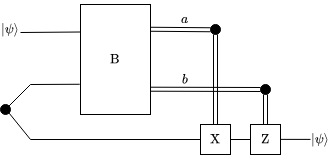
\includegraphics[width=0.75\linewidth]{body/ch3/figs/chuang-teleportation}
	\caption[Quantum Circuit for Quantum Teleportation by Chuang and Gottesman.]{This quantum circuit demonstrates how quantum teleportation uses measurements to transfer states from on place to another \cite{gottesman1999demonstrating}. The symbol with the black dot and diverging wire to the left of the circuit represents an EPR state and the box $B$ represents a Bell measurement of the input states. Double lines represent classical outputs.}
	\label{fig:chuang-teleportation}
\end{figure}

In order for sender A to convey $n$ bits of information to the receiver B, \textit{Holevo's theorem} states that, where quantum entanglement is available and qubit communication in either direction is permitted, A must send B at least at $\lceil n/2 \rceil$ qubits \cite{cleve1998quantum, holevo1998quantum}. Holevo's theorem holds regardless of the prior entanglement and communication from B to A \cite{cleve1998quantum}. A consequence of Holevo's theorem is that a low-dimensional quantum computer, with a small number, cannot contain too much accessible information \cite{DeWolf2019}. Another consequence of Holevo's theorem that was derived by Cleve et al. and elaborated on by de Wolf can be demonstrated using the case where sender A wants to communicate a string $x$ to receiver B \cite{cleve1998quantum, DeWolf2019}. If A sends $m$ qubits to B, and both parties did not share some prior entangled state, then B receives at most $m$ bits of information about $x$ \cite{cleve1998quantum, DeWolf2019}. Conversely, if A sends B $m$ qubits, and they share some prior entangled state, then B receives at most $2m$ bits of information about string $x$ \cite{cleve1998quantum, DeWolf2019}. Furthermore, if A sends B $m$ classical bits, and they shared some prior entangled state, then B receives at most $m$ bits of information about $x$ \cite{cleve1998quantum, DeWolf2019}. Thus, despite having $2^m$ complex amplitudes, an $m$-qubit quantum computer is no better at potentially storing or transmitting information than a classical computer with $m$-bit wide registers and communication channel bandwidths \cite{DeWolf2019}. However, prior entanglement can improve the performance of quantum communication when superdense coding properties are considered \cite{DeWolf2019}. Additionally, by sharing prior entangled states, the qubit on the sender's side is destroyed, which prohibts unknown qubits from being copied in a quantum computer \cite{DeWolf2019}.

\subsection{Communication in Quantum Key Distribution Networks}

According to an artical by Wootters in 1982, cloning qubits is prohibited by linearity of quantum mechanics \cite{wootters1982single}. The no-cloning property of qubits makes quantum computers suitable for cryptography and secure communication. In particular, the principles of quantum communication explored here are useful for Quantum Key Distribution (QKD) networks. The goal of QKD is to allow point-to-point communication between two remote parties linked by a quantum channel and an authenticated classical channel to share a common random binary string known as a \textit{key} \cite{salvail2010security}.  According to Salvail et al., a QKD network is an infrastructure that is capable of performing long-distance and high-rate secret key agreements \cite{salvail2010security}. QKD networks perform key establishment methods which are based on protocols, including locally executed algorithmic steps and public communication \cite{salvail2010security}. 

A QKD network developed by the Secure Communication based on Quantum Cryptography (SECOQC) project in consists of node modules which enable authentic classical communication required for key distillation, manages the generated key material, determines a communication path between any destinations in the network, and establishes secure transport of key material between destinations \cite{peev2009secoqc}. The network topology of the SECOQC QKD network consists of a Coherent One-Way (COW) time coding system that uses a novel distributed phase reference COW protocol to enable communication for up to $\SI{85}{\kilo\meter}$ \cite{peev2009secoqc}. At the start of the protocol, the sender prepares pulses of weak coherent states using a Continuous-Wave (CW) laser with a wavelength of $\SI{1550}{\nano\meter}$ and an intensity modulator \cite{peev2009secoqc}. The logical bits 0 and 1 are encoded in two-pulse sequences, which can be written as a product of coherent states $\ket{\sqrt{\mu}}$ and $\ket{\sqrt{0}}$ such that the $k$-th logical qubit is given by
\begin{align}\label{eqn:secoqc-kth-bit}
	\ket{0_k}	& = \ket{\sqrt{\mu}}_{2k-1} \ket{\sqrt{0}}_{2k}\nonumber\\
	\ket{1_k}	& = \ket{\sqrt{0}}_{2k-1} \ket{\sqrt{\mu}}_{2k}
\end{align} 
These encoded states are not orthogonal, however, a conclusive ToA measurement can provide the optimal unambiguous determination of the bit value \cite{gisin2004towards}.

Pulses propagate to receiver B through a quantum channel characterised by a transmission channel $t$ and are separated at a beamsplitter with a transmission coefficient $t_B \leq 1$ such that only $10\%$ of the pulses are reflected into B's \gls{interferometer} to check for quantum state coherence \cite{peev2009secoqc}. Due to the large coherence times of the CW laser, there is a well-defined phase between any two non-empty pulses across the bit separation and within decoy sequences. The receiver measures the time-of-arrival (ToA) of these pulses to provide an unambiguous determination of bit values and establish the raw key. The COW QKD system can detect an attack by an eavesdropper by using InGaAs single-photon laser diodes operating with an intensity modulator to produce signal and decoy pulses that can be measured behind an \gls{interferometer} as illustrated in figure \ref{fig:cow-protocol} \cite{peev2009secoqc}. To ensure security, the wavelength of A's laser is adjusted in a way that only one of two monitoring detectors at the receiver is triggered \cite{peev2009secoqc}. 
\begin{figure}[!ht]
	\centering
	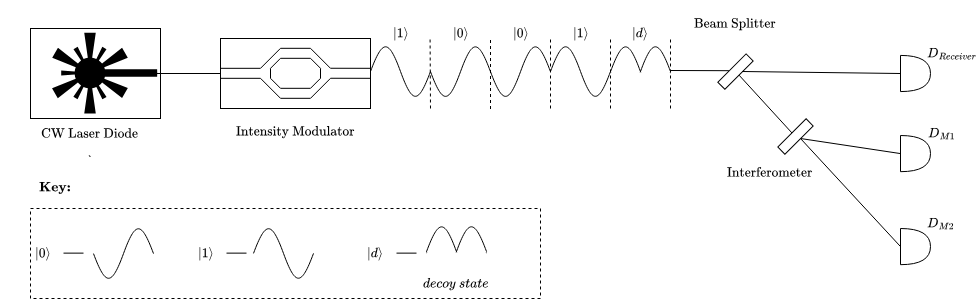
\includegraphics[width=1.0\linewidth]{body/ch3/figs/cow-protocol}
	\caption[Coherent One-Way (COW) Quantum Key Distribution System by GAP University of Geneva.]{The sender's CW laser and intensity modulator are illustrated on the left and the receiver's InGaAs detectors are illustrated to the right. The COW QKD system's CW laser has large coherence length to prevent phase-shift and photon number splitting attacks by producing a well-defined phase between two non-empty pulses across a bit sequence and within a decoy sequence \cite{peev2009secoqc}. Pulses propagate through a quantum channel to InGaAs detectors at the receiver. The main receiver detector $D_{Receiver}$ checks quantum coherence, while detectors $D_{M1}$ and $D_{M2}$ ensure security by revealing any action by an eavesdropper.}
	\label{fig:cow-protocol}
\end{figure}
The SECOQC QKD network also includes a one-way weak pulse system implemented by Toshiba Research Europe Ltd (TREL) that transmits optical pulses with a wavelength of $\SI{1.55}{\micro\meter}$ along a quantum channel at a repetition rate of about $\SI{7}{\mega\hertz}$ \cite{peev2009secoqc}. TREL used strong clock pulses with a duration of $\SI{5}{\nano\second}$ each and that do not overlap with the signal pulses to establish synchronisation between the different parts of the system \cite{peev2009secoqc}. An intense modulator is used to produce decoy sequences that are strongly attenuated to the single-photon level and the strong clock pulse is multiplexed with the decoy pulses to provide synchronisation \cite{peev2009secoqc}. The receiver uses two single-photon InGaAs avalanche photodiodes (APDs) as detectors that are adjusted to avoid fake-state attacks and time-shift attacks \cite{peev2009secoqc}. The receiver cannot use a modulator or optical attenuator to secure the system because the attenuator would absord a large percentage of all the single photons from the sender \cite{lydersen2011secure}. Fake-state attacks exploit the classical photodiode mode of the APD by triggering the detector in the presence of bright pulses \cite{lydersen2011secure}. 

\subsection{Methods for Preventing Fake-Attacks and Time-Shift Attacks}

Lydersen et al. proposed background illumination to keep the APDs in the classical photodiode mode so that the detectors only respond to bright optical trigger pulses and not single-photons \cite{lydersen2011secure}. Fake-attacks can also be prevented by using gated APDs whose single-photon sensitivity is based on measurements of time-of-arrival. Time-shift attacks are based on detector efficiency mismatch (DEM) in the time-domain \cite{lydersen2011secure}. For example, if the receiver B's apparatus contains two single-photon detectors (SPDs) for incoming photons - one for each bit value - the detection windows and hence the efficiency curves of the two detectors would be slightly shifted \cite{lydersen2011secure}. Lydersen et al. performed an experiment where an eavesdropper E was able to capture partial information about the key in $4\%$ of all time-shift attacks attempts \cite{lydersen2011secure}. For a short SECOQC QKD fibre link of $\SI{1}{\kilo\meter}$, TREL were able to achieve a high secure bit rate of $\SI{27}{\kilo\bit\per\second}$ for $24$ hours \cite{peev2009secoqc}. 

A QKD system that exploits entanglement was developed by an Austrian-Swedish consortium for generating secure keys as part of the SECOQC QKD network \cite{peev2009secoqc}. The schematic of the system in figure \ref{fig:ent-qkd} shows the optical and electronic connections between the different components. When the system is initialised, the entanglement source at sender A's location produces polarisation-entangled photon EPR pairs at $\SI{810}{\nano\meter}$ and $\SI{1550}{\nano\meter}$ \cite{peev2009secoqc}. The $\SI{810}{\nano\meter}$ photon is detected using four silicon-based APDs with four phase-encoded polarisation basis states $\{\ket{-\pi/4}$,$\ket{0}$,$\ket{\pi/2}$,$\ket{\pi/4}\}$ while the $\SI{1550}{\nano\meter}$ photon is transmitted to receiver B using single-mode fibres (SMF) \cite{peev2009secoqc}. The $\SI{1550}{\nano\meter}$ photon of the EPR pair travels through the quantum channel with low transmission losses and is registered by the receiver using passive polarisation analysers with four InGaAs avalanche photodiodes \cite{peev2009secoqc}. The receiver uses FPGAs to analyse the synchronised pulse arriving at four InGaAs-APDs with the same phase-encoded polarisation states \cite{peev2009secoqc}. 
\begin{figure}[!ht]
	\centering
	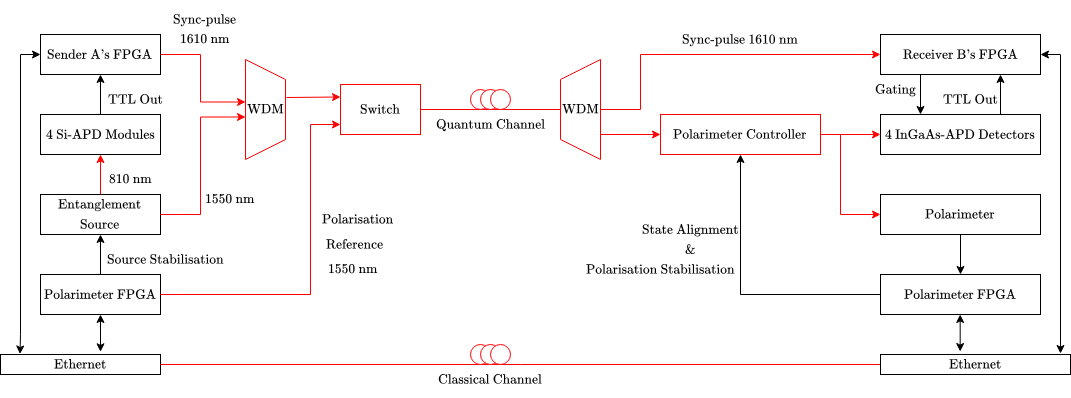
\includegraphics[width=1.0\linewidth]{body/ch3/figs/ent-qkd}
	\caption[Schematic of the Ent Quantum Key Distribution System in the SECOQC Network by the Austrian Institute of Technology at the University of Vienna.]{The Ent QKD system generates a secure key using Bell state measurements of entangled qubits at the location of the transmitter and the receiver. The source creates polarisation entangled photon pairs at highly non-degenerate wavelengths which are locally analysed in four polarisation states. FPGAs are used to process all detection events and logged onto computers \cite{peev2009secoqc}.}
	\label{fig:ent-qkd}
\end{figure}
More FPGAs are used to control the source stabilisation module at the sender's location as well as for implementing \gls{polarimeter} modules at both ends of the point-to-point communication \cite{peev2009secoqc}. The source stabilisation modules use automatically adjusted \gls{piezo-actuated} fibre couplers to achieve maximum photon detection rates to ensure that the photon flux emitted from the crystal is efficiently coupled to the SMFs leading to the detectors at A and B \cite{peev2009secoqc}. Polarimeter modules control the polarisation to ensure that the QKD system produces a reliable and stabilised distribution of phase-encoded qubits in the optical fibre-based quantum channels \cite{peev2009secoqc}. Similar to the COW QKD system, the Ent QKD system synchronises the trigger signals used to gate the receiver's InGaAs-APDs must be synchronised to initialise the detection window when a single photon is expected \cite{peev2009secoqc}. 

\section{Bit Mapping and Qubit Mapping for Quantum Computing Hardware Platforms}

When referring to APDs, Lydersen et al. use the term 'gated' to refer to the ability of an APD detector to be single-photon sensitive only when a photon is expected to arrive, i.e. in the detection window \cite{lydersen2011secure}. Lydersen et al. employed the concept of gating detectors to present a method for securing Bob's receiver called \textit{bit-mapped gating} which protects the system against pulses from regions that are outside the central neighbourhood of the detector gate in the implemented protocol \cite{lydersen2011secure}. Bit-mapped gating is implemented in software to determine how the signals from detectors $a$ and $b$ are mapped into the logical bits $0$ and $1$ \cite{lydersen2011secure}. Optical bit mapping defines the relationship between the detectors, $a$ and $b$, and the quantum states with qubit values $\ket{0}$ and $\ket{1}$ in the $Z$ basis \cite{lydersen2011secure}. Software and optical bit mapping need to coincide in order to ensure that the bit value sent by A matches the value received by B. 

\subsection{Optical Bit Mapping}

Bit-mapped gating is implemented between the detector gates and begins with receiver B randomly assigning detectors $a$ and $b$ values of 0 and 1 \cite{lydersen2011secure}. Following the selection of the software bit mapping, the basis is selected randomly between the $X$ basis which corresponds to the $\pi/2 \si{\radian}$ phase shift and the $Z$ basis corresponding to the $0 \si{\radian}$ phase shift along with random optical bit mapping \cite{lydersen2011secure}. Figure \ref{fig:optical-bit-mapping} shows an example of a timing diagram used by Lydersen et al. to represent possible optical bit mapping schemes \cite{lydersen2011secure}.
\begin{figure}[!ht]
	\centering
	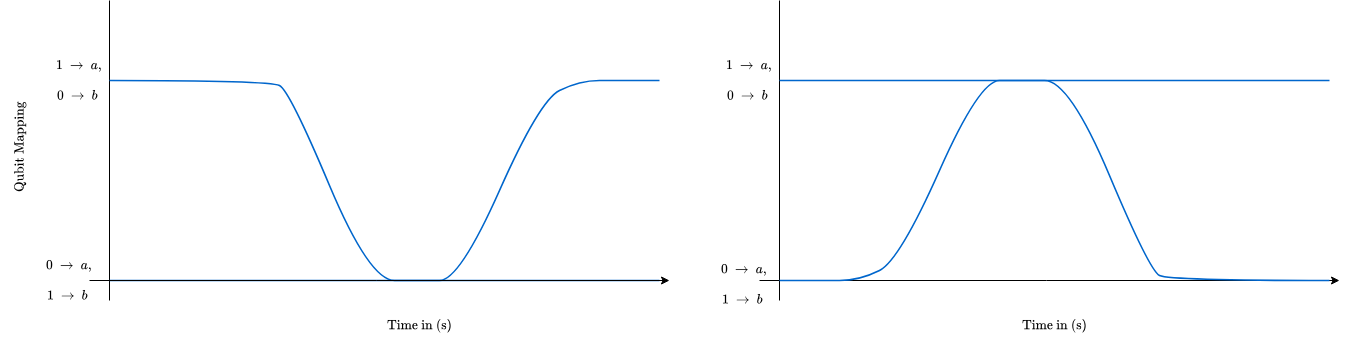
\includegraphics[width=1.0\linewidth]{body/ch3/figs/optical-bit-mapping}
	\caption[Timing Diagram for Possible Optical Bit Mapping Scheme by Lydersen et al.]{Showing possible optical bit mappings corresponding to $0$ and $\pi$ phase shift in one basis, and $\pi/2$ and $3\pi/2$ in the opposite basis \cite{lydersen2011secure}.}
	\label{fig:optical-bit-mapping}
\end{figure}
Lydersen et al. noted that in a phase-encoded system, the two levels would correspond to a phase of $0$ and $\pi \si{\radian}$ \cite{lydersen2011secure}. Detector gates facilitate software and optical bit mapping correspondence \cite{lydersen2011secure}. A bit-mapped gate refers to the period of matching optical and software bit mapping \cite{lydersen2011secure}. The aim of bit mapping is to ensure that all states received and detected outside the bit-mapping gate cause random detection results by applying randomised selection in optical and software bit mapping, and thereby improving the security of a QKD system \cite{lydersen2011secure}. Detections in the middle of the gate produce a quantum bit error rate (QBER) of $0\%$, whereas detections outside the centre produce a QBER of $50\%$ \cite{lydersen2011secure}. Lydersen et al. also showed that multiple photons detected individually in a single optical mode, corresponding to the ToA $t$, increase the minimum QBER \cite{lydersen2011secure}. This can be accounted for by the fact that when each photon hits a separate set of detectors and the detection results are merged to give the detection results of threshold detectors \cite{lydersen2011secure}. 

\subsection{Differentiating Between Physical Qubits and Logical Qubits}

In the application of quantum computers for approximate combinatorial optimisation, Farhi et al. differentiated between a \textit{physical qubit} from a \textit{logical qubit} to employ a sequence of parametrised unitary operations that sit on the qubit layout to produce quantum states based on the parameters  \cite{farhi2017quantum}. In essence, a logical qubit is a physical or abstract qubit that forms part of a quantum algorithm or quantum circuit and is mapped onto a physical qubit, which is a quantum particle or device whose behaviour can be described by the $\ket{0}$ and $\ket{1}$ basis state \cite{zhang2021time}. Alternatively, the quantum computer can produce quantum states whose discretised energy is near the ground state energy of a given quantum-well with a given Hamiltonian $H$ \cite{farhi2017quantum}. Ultimately, both implementations of quantum computers satisfy DiVincenzo's criterion for initialising a qubit to a ground state $\ket{0}$ \cite{farhi2017quantum, divincenzo2000physical}. Furthermore, the quantum computers both have a sequence of universal unitary transformations that act on the initial state to produce a desired quantum state $\ket{\mathbf{\nu}}$ that depends on the eigenvalues and linear coefficients of the unitary operations \cite{farhi2017quantum}. Given $L$ unitary operations, corresponding to $L$ quantum gate operations, Farhi et al. write the desired state as, 
\begin{align}\label{eqn:desired-state-from-initial}
	\ket{\underline{\nu}} & = U_L(\nu_L)\cdots U_1(\nu_1)\ket{0}
\end{align} 
where $\mathbf{\nu}$ denotes the collection $\nu_1,...,\nu_L$ of parameters and each quantum gate operation $U_i$ depends on this set of parameters \cite{farhi2017quantum}. The aim of the combinatorial optimisation quantum algorithm is to choose the parameters $\mathbf{\nu}$ such that the expected value of the objective function $C$ is maximised or such that that the expected value of the Hamiltonian $H$ is small \cite{farhi2017quantum}. An $n$ qubit quantum computer produces states as shown in \ref{eqn:desired-state-from-initial} and a classical optimisation routine that takes as input, a sequence of parameters $\mathbf{\nu}$ associated with maximal expectation values and outputs a new value of the parameters \cite{farhi2017quantum}. The pseudocode of the algorithm takes a classical objective function $C$ on $n$ strings that can efficiently be evaluated on any input string $z$ as the input \cite{farhi2017quantum}. 

In the procedure, a repetition number $R$ is selected along with a stopping criterion which may depend on the quality of the objective function value or the number of clock cycles of the quantum computers. Then, the quantum computer is started by initialising the ground state and one of the $n!$ ways of assigning the $n$ bits associated with the objective function to the physical qubits \cite{farhi2017quantum}. After selecting the initial set of parameter in the collection $\mathbf{\nu}$, the algorithm runs until for $R$ times or until the stopping criterion is satisfied. In loop, a measurement is performed in the computational basis which produces a string $z$ for evaluating the objective function $C$ \cite{farhi2017quantum}. Finally, the algorithm outputs the string $z$ with the highest value of $C(z)$. Farhi points out that although it suffices to only consider objective functions that can be written as a sum of individual terms involving two classical bits, the connectivity of the objective function may have nothing to do with the pairwise connectivity of physical qubits in the hardware \cite{farhi2017quantum}. 

Qubit pairs that can be acted on by two-qubit gates depend on the hardware architecture \cite{farhi2017quantum}. The qubits on the hardware can also be labelled as $\ket{1}_{10}$,...,$\ket{n}_{10}$, corresponding to the total number of qubits of the quantum computer. In the space-time volume of a quantum computation, Farhi et al. arrange $n$ qubits in a $\sqrt{n}\times \sqrt{n}$ grid array which is initialised by preparing the quantum state of each qubit \cite{farhi2017quantum}. Each qubit is coupled to 4 other qubits except at the borders of the grid. Layers of single-qubit gates and two-qubit gates act on the qubits with operations that are restricted by the hardware architecture \cite{farhi2017quantum}. 

\subsection{Modelling Quantum Computers with Physical and Logical Qubits}

In a similar study of the qubit mapping problem, Li, Ding and Xie suggest that based on a given quantum circuit and the coupling information of the device, a quantum computing solution requires an initial logical-to-physical qubit mapping and an intermediate mapping transition which is able to remap two logical qubits in a two-qubit gate to two coupled physical qubits \cite{li2019tackling}. Li et al. developed a flexible \texttt{swap} gate-based heuristic algorithm, called SABRE, for finding the optimal solution to the qubit mapping problem which is applicable to Noisy Intermediate-Scale Quantum (NISQ) devices with arbitrary connections between qubits \cite{li2019tackling}. Li et al. noted that for NISQ devices, such as the IBM Q20 quantum processor, the assumption that two-qubit gates can be applied to arbitrary two logical qubits in a quantum algorithm does not hold \cite{li2019tackling}. This is because when running a quantum program, logical qubits need to be mapped to the physical qubits, analogous to register allocation in classical computing but for physical qubits NISQ devices, a qubit can only couple with its nearest neighbour so that for a specific mapping, two-qubit pairs can only be applied to limited logical qubit pairs \cite{li2019tackling}. Therefore, a quantum circuit cannot be directly implemented on NISQ devices \cite{li2019tackling}. To resolve this limitation of NISQ devices, qubit mappings and circuit transformations are required to make the circuit compatible during compilation \cite{li2019tackling}. 
   
According to the \textit{Gottesman-Knill theorem}, a computation that involves state operations in the computational basis, Hadamard gates, phase gates, controlled-\texttt{NOT} gates, single-qubit Pauli gates, and measurements of observables in the Pauli group, may be simulated efficiently on a classical computer \cite{Nielsen2010}. Li et al. exploited this fact to develop the SABRE algorithm with the observation that effective mapping transition needs to start from the qubits in the two-qubit \texttt{CNOT} gates that need to executed on an IBM 20-qubit chip model \cite{li2019tackling}. Before extending the application of the algorithm to 20 qubits, Li et al. use a small-sized 4-qubit device model as the hardware platform as an example for demonstrating initial logical-to-physical qubit mappings. In the 4-qubit device model, two-qubit gate operations are only allowed on the physical qubit pairs $\{Q_1, Q_2\}$, $\{Q_2, Q_4\}$, $\{Q_3, Q_4\}$ and $\{Q_1, Q_3\}$ \cite{li2019tackling}. Assuming that the initial logical-to-physical qubits mapping is $\{q_1 \rightarrow Q_1, q_2 \rightarrow Q_2, ...\}$, the execution of a quantum circuit with six \texttt{CNOT} gates to the device requires only four out of the six gates because the fourth and the sixth gates cannot be executed since the corresponding qubits are not coupled \cite{li2019tackling}. 

The SABRE algorithm approximates a perfect initial mapping to satisfy all two-qubit gate dependencies by employing \texttt{swap} gates that change the qubit mapping by exchanging states between two qubits to make all \texttt{CNOT} gates executable without changing the overall functionality of the circuit \cite{li2019tackling}.  The use of \texttt{swap} gates increases the number of operations in the circuit which carry imperfections that introduce noise and hence, the overall error rate \cite{li2019tackling}. Additionally, introducing \texttt{swap} gates to the qubit mapping increases the circuit depth, which leads to an increase in the total execution time and error accumulation from qubit decoherence \cite{li2019tackling}. Three \texttt{swap} gates are introduced in the initial qubit mapping, increasing the total number of gates in the circuit from $6$ to $9$ gates and increasing the circuit depth from $5$ to $8$ \cite{li2019tackling}. Figure \ref{fig:li-qubit-mappings} illustrates the original quantum circuit with 6 \texttt{CNOT} gates alongside the updated hardware-compliant quantum circuit with 3 additional \texttt{swap} \cite{li2019tackling}. 

\begin{figure}[!ht]
	\centering
	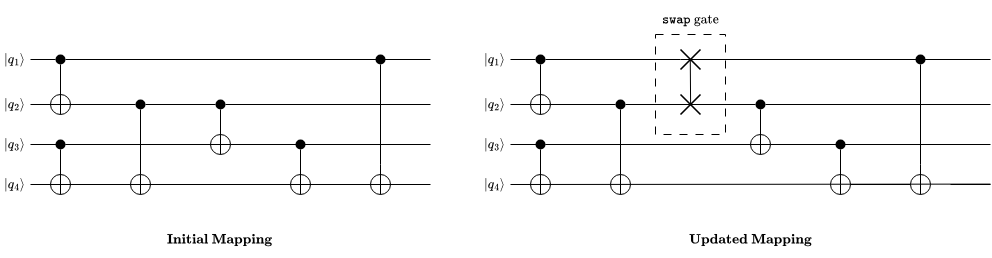
\includegraphics[width=1.0\linewidth]{body/ch3/figs/li-qubit-mappings}
	\caption[Hardware-Compliant Quantum Circuit for a 4-qubit Device by Li et al.]{In their article, Li et al. proposed the used of \texttt{swap} gates to change the qubit mappings to allow all the \texttt{CNOT} gates to circumvent the logical-to-physical qubit mapping problem where corresponding qubit pairs are not connected. \cite{li2019tackling}.}
	\label{fig:li-qubit-mappings}
\end{figure}

Li et al. implemented the SABRE algorithm in the Python coding language without any parallelisation or acceleration \cite{li2019tackling}. The heuristic search experiments were executed on a server with Intel Xeon E5-2680 CPUs containing 48 logical cores each and $\SI{48}{\giga\byte}$ of memory. Compared to other algorithms such as Zulehner et al.'s Best Known Algorithm (BKA) which required $\SI{40}{\giga\byte}$ memory and $\SI{474.81}{\second}$ execution time, the SABRE algorithm was observed to be more efficiency, requiring about $\SI{200}{\mega\byte}$ memory and $\SI{0.08}{\second}$ runtime \cite{li2019tackling, zulehner2018efficient}. Zulehner et al.'s BKA algorithm differs from the SABRE algorithm in that it searches all possible combinations of \texttt{swap} gates that can be applied concurrently to minimize the output circuit depth and the number of additional \texttt{swap} gates at the same time which requires $\mathcal{O}$, whereas the SABRE algorithm uses a heuristic cost function to help find the \texttt{swap} that can reduce the sum of distances between each qubit pair in the front layer \cite{zulehner2018efficient, li2019tackling}.  

The metrics for evaluating the qubit mapping efficiency discussed above, including the QBER, total number of quantum gates used, quantum circuit depth, memory usage and execution time form an essential part for benchmarking the FPGA-based emulated quantum computing system. The following section discusses existing frameworks for emulating the different properties of quantum computers on FPGA-based hardware accelerators.

\section{Representations of Qubits in FPGA-Based Quantum Computer Emulations \label{sec:lit-qubit-rep}}

While studying the emulation of quantum systems on FPGA, Minoru Fujishima noted that realisation of a quantum computer with large-scale qubits is difficult in both physical quantum mechanical processes and software simulation \cite{fujishima2003fpga}. The quantum state of a qubit is directly related to the complex and real parts of the normalised amplitude coefficients in the linear combination of the state vectors $\ket{0}$ and $\ket{1}$ which collapse to a single value depending on the magnitude of the probabilistic complex coefficient. As the number of qubits $n$ in the system is increased, the computational requirements for storing and manipulating the $2^n \times 2^n$ dense matrices involved in quantum algorithms also increased. To efficiently model qubits in the FPGA-based emulation, careful consideration needs to be taken on the design and implementation of qubits and a concise methodology needs to be defined for the transformations that can be performed on them. Typically, emulations of quantum computers on FPGA focus on optimising the storage and manipulation of the complex coefficients as fixed-point or floating-point numbers \cite{Aminian2008, Hlukhov2021, Khalid2004, Khalil2015}.  

\subsection{Assigning Probabilities to Input-and-Output Tables}

The focus of Fujishima's study was in solving \gls{NP-complete} problems in polynomial time using a quantum computer. In finding solutions to NP-complete problems with output $y = f(x)$, the aim is to find the input $x$ for the output $y$. To solve problems of this class, Fujishima used the QFT in Shor's algorithm to find the solution for periodic input-and-output pairs in polynomial time \cite{fujishima2003fpga}. When the input-and-ouput pairs of the system were not periodic, Fujishima noted that using Grover's search algorithm increased the computational time proportional to the square root of the number of input-and-output pairs \cite{fujishima2003fpga}. 

Fujishima assigned separate qubits for the input $x$ and the output $y$ such that all the output registers correspond to input registers and the same qubit cannot be used foar an output and an input \cite{fujishima2003fpga}. For example, a simple 2-qubit quantum computer with 2 input registers and 2 corresponding output quantum registers is shown in figure \ref{fig:fujishima-inout} where the input and output qubits for generating the input-and-output table are labeled $\ket{q_0q_1}$, and $\ket{q_2q_3}$, respectively \cite{fujishima2003fpga}. Separate qubits were added during the calculation according to the number of ancilla qubits required in the quantum algorithm \cite{fujishima2003fpga}. To optimise the emulation pipeline, Fujishima dealt with qubits using two different approaches, namely, a logic quantum processor (LQP) and a quantum index processor (QIP). 

\begin{figure}[!ht]
	\centering
	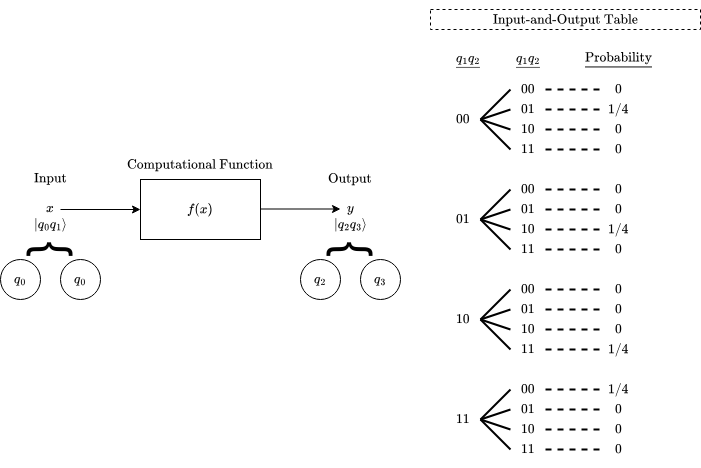
\includegraphics[width=1.0\linewidth]{body/ch3/figs/fujishima-inout}
	\caption[Input-and-Output Table by Fujishima.]{In the first stage of the FPGA-based emulation pipeline proposed by Fujishima, the input-and-output table is generated to solve an NP-complete problem with input $x$ and output $y=f(x)$ using a quantum computer. Fujishima suggests that the qubit input-and-output table shown needs to be generated in polynomial time \cite{fujishima2003fpga}.}
	\label{fig:fujishima-inout}
\end{figure}

Fujishima noted that for the quantum algorithm to be executed in polynomial time, the table of input-and-output qubit pairs should also be generated in polynomial time. This can by achieved by encoding information in the period of the outputs of the input-and-output table prior to the first step of the emulation pipeline \cite{fujishima2003fpga}. The first step of the emulation pipeline that uses a logic process distributes the probabilities equally to the quantum states corresponding to the candidate answer in the quantum search algorithm that finds the correct input-and-output pair in the table \cite{fujishima2003fpga}. Only two probabilities appear in the table, i.e. 0 and $1/m,~~m\in\mathbb{Z}^+$, before the second stage \cite{fujishima2003fpga}. 

In each case, the number $m$ corresponds to the number of entries in the input-and-output table. Thus, using the different registers for the input and output allowed Fujishima to design a LQP that expresses probabilities in binary \cite{fujishima2003fpga}. The QIP was developed to improve memory usage by observing that the output depends on the location of 1 in the quantum states used as inputs to the input-and-output table \cite{fujishima2003fpga}. Fujishima designated the term quantum index to refer to the location of 1 in the QIP. To illustrate the difference in the amount of memory used by the QIP compared to the LQP in order to process quantum states, Fujishima used the illustration in \ref{fig:fujishima-lqp-qip}, showing that the QIP is only required to store half the number of quantum states related to the candidate solution in the input-and-output table \cite{fujishima2003fpga}. 

\begin{figure}[!ht]
	\centering
	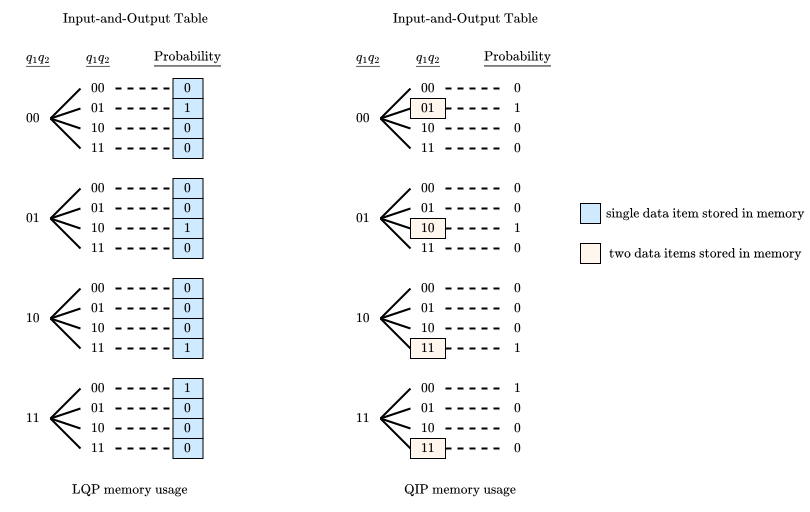
\includegraphics[width=1.0\linewidth]{body/ch3/figs/fujishima-lqp-qip}
	\caption[Memory Comparison for Logic Quantum Processor (LQP) and Quantum Index Processor (QIP).]{In comparison, the LQP uses more memory than the QIP for the same input-and-output table. An LQP implementation requires all probabilities to be stored in memory, whereas the QIP only stores the quantum index.}
	\label{fig:fujishima-lqp-qip}
\end{figure}

A FPGA with 1.5 million gates was used to implement a QIP with 2048 processing elements, corresponding to 11 qubits \cite{fujishima2003fpga}. Each processing element was driven by a clock at $\SI{80}{\mega\hertz}$ and consisted of logic unit, a memory block and a temporary register as illustrated in figure \ref{fig:fujishima-qip-block}. Qubit errors were modelled at high speed by generating quantum NOT operations stochastically. Furthermore, each processing element contained 64 qubits, making a total of 75 qubits for the implementation of the QIP. Using the QIP, the computation time increased by a factor of $10^{18}$ compared to the implementation of the LQP \cite{fujishima2003fpga}. The shortcoming of Fujishima's study is that the results do not show the overall memory usage for the proposed LQP and QIP designs.  

\begin{figure}[!ht]
	\centering
	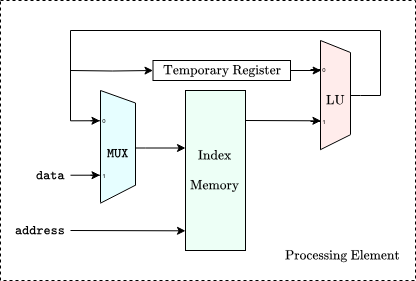
\includegraphics[width=1.0\linewidth]{body/ch3/figs/fujishima-qip-block}
	\caption[Fujishima's Processing Element for Emulating Qubits.]{The QIP processing element for emulating the parallel computing of quantum states in a quantum computer. Fujishima implemented 2048 processing elements for executing the calculations using quantum indices in the input-and-output table. \cite{fujishima2003fpga}.}
	\label{fig:fujishima-qip-block}
\end{figure}

\subsection{Representing Qubit Probabilities Using A Fixed-Point Scheme with Mantissa Bits}

Khalid, Zilic and Radecka were able to expand on the study by Fujishima by proposing a new FPGA-based emulator design that allows efficient experimentation with new quantum algorithms. Khalid et al.'s paper concentrated on new techniques for modelling quantum circuits, including entanglement and probabilistic computing realisation \cite{Khalid2004}. The primary difference between Fujishima's approach and Khalid et al.'s approach is that unlike Fujishima who used an input-and-output table, Khalid et al. considered the probabilistic nature of quantum states which leads to measurement error \cite{Khalid2004}. In addition, Fujishima's study did not include results from the synthesised circuit on a FPGA. To integrate the probabilistic nature of qubits while managing resources for emulating quantum circuits efficiently on an Altera Stratix EP1S80B956C6 FPGA, Khalid et al. used a fixed-point scheme to represent the values of the normalised amplitudes $\alpha$ and $\beta$ which represent the probability of measuring one of the basis states. To perform quantum measurements, Khalid et al. proposed that it suffices for the probabilities of detecting each state to be pre-computed in software and stored in hardware. These probabilities can be used as weights to emulate the random state detection in hardware \cite{Khalid2004}. 

Khalid et al. highlighted that a classical probabilistic circuit runs a series of inputs through the network of gates and outputs the bits according to the probability distribution induced by the network \cite{Khalid2004}. This leads to the probability of an error in measuring probabilistic circuit outputs.  Khalid et al. elucidated that the choice of a fixed-point scheme over a floating-point scheme was due to the fact that $\alpha$ and $\beta$ can have a decimal point of 0 or 1 only, as shown in the theoretical framework in section \ref{subsec:qft} \cite{Khalid2004}. Khalid et al. further elaborated that using a floating-point representation of the complex exponent does not bring benefits in this case \cite{Khalid2004}. To achieve precision, Khalid et al. used \gls{mantissa} bits in a modular way by changing the size of the fractional part without modifying other components of the system. This method is advantageous for experiments dealing with precision and fault-tolerance of quantum algorithms and incorporates the ideas of error correction to the emulator \cite{Khalid2004}. 

\subsection{Emulation Accuracy and Logic Cell Usage}

In a similar 2008 study of an FPGA-based quantum circuit emulation, Aminian et al. proposed a new representation for qubits to considerably improve the application of quantum circuits on FPGA-based emulations \cite{Aminian2008}. Aminian et al. represented complex coefficients of each qubit using fixed-point numbers with an $N$ bit \gls{mantissa}. Given that a qubit in the computational basis has two complex coefficients with two components each, four fixed-point numbers were used to represent a qubit \cite{Aminian2008}. Amina et al. noted that the emulation accuracy of the design was directly related to the number of mantissa bits for measuring the emulation efficiency. The emulation accuracy increased as the number of \gls{mantissa} bits is increased \cite{Aminian2008}.

The results from Aminian et al.'s implementation were compared to the implementation by Khalid et al. to estimate the overall improvement in the usage of logic cells when different mantissa bit-sizes were implemented. When Aminian et al. performed the emulation experiments on an Altera Stratix EPIS80B9056C6 FPGA, the results showed a higher improvement in the usage of logic cells for the implementation that uses an 8-bit mantissa \cite{Aminian2008}. Aminian et al. were particularly interested in the logic cell usage for different qubit transformations using Hadamard, phase shift, Pauli, and \texttt{CNOT} quantum gates. Experimental results showed the best improvement ($99\%$) in logic cell usage from Khalid et al.'s implementation when the \texttt{CNOT} operation was performed \cite{Aminian2008}. This improvement corresponded to employment of a 16-bit mantissa to perform the unitary matrix operation. In this case, Khalid et al.'s implementation of the \texttt{CNOT} used 375 logic cells, but Aminian et al. required only 4 logic cells in their implementation \cite{Aminian2008}.

\subsection{Representing Qubits on a Bloch Sphere To Emulate Entanglement Using VHDL}
  
In 2008, Mohamed, Badawy and Jullien, investigated how a programmable logic array could be used to practically emulate quantum computations with entanglement characteristics by extending the concept of phase and the Bloch sphere representation of qubits to classical bits on a FPGA \cite{mohamed2009using}. Mohamed et al. emphasised that apart from the initial set of quantum states and the final measured state, the hidden state of a qubit must also be stored by a classical computer in two complex fixed-point registers representing a qubit on the surface of a Bloch sphere \cite{mohamed2009using}. Assuming that a 10-bit fixed-point number representation is sufficient precision for the coefficients, then 40 bits of classical storage are required to represent the quantum state of one qubit \cite{mohamed2009using}. Mohamed et al. underscored that two parameters may be used to represent a qubit by observing that, by expressing an internal qubit state as the density matrix
\begin{align}\label{eqn:density-matrix}
	\rho	& = \frac{1}{2}\left(I + \beta_x\sigma_x + \beta_y\sigma_y + \beta_z\sigma_z\right)
\end{align}
where $\beta_x$, $\beta_y$ and $\beta_z$ are real numbers and $I$, $\sigma_x$, $\sigma_y$, and $\sigma_z$ are Pauli matrices, the spherical coordinates $r$, $\phi$ and $\theta$ could be used with $r = 1$ from the normalise constraint which requires that
\begin{align}
	\beta_x^2 + \beta_y^2 + \beta_z^2 = 1\nonumber
\end{align}
Mohamed et al. used this approach to represent a qubit as a vector on the surface of a Bloch sphere. This implementation ignored the overall phase factor of the qubit since it is not observable, even though the factor appears general mathematical representation of the coefficients in spherical coordinates given by
\begin{align}\label{eqn:qubit-spherical-coordinates}
	\alpha_0	& = e^{i\gamma}\cos(\theta/2)\\
	\alpha_1  & = e^{i\gamma}e^{i\phi}\sin(\theta/2)
\end{align}
In this form, the spherical coordinate representation of a qubit is only applicable to a single qubit quantum computer, which cannot be more useful than a single bit classical computer in terms of its computational capabilities. Recalling that for a two-qubit quantum computer, the state of the system is related by the basis vectors $\ket{00}, \ket{01}, \ket{10}, \ket{11}$, it can be observed that the internal state of two qubits requires representation by 4 complex fixed-point registers or 7 floating-point numbers \cite{mohamed2009using}. Mohamed et al. generalised this observation by suggesting that the internal state of a quantum register with $n$ qubits requires $2\times2^n - 1$ classical fixed-point registers \cite{mohamed2009using}.

While conducting experiments on a FPGA, the representation of a qubit using the angles $\theta$ and $\phi$ was achieved using LUTs for managing the $\sin$ and $\cos$ functions and manipulation of the complex coefficients $\alpha_{0}$ and $\alpha_{1}$ \cite{mohamed2009using}. This representation of qubits in spherical coordinates is suitable for the operations on the qubits that result in state vector rotations on the surface of a Bloch sphere or unit circle. According to Mohamed et al., the number of entries in the LUT is a function of the angle resolution and the number of bits per entry is a function of the required precision of the representation of the sinusoidal functions \cite{mohamed2009using}. Since the ratios produced by the sine function in the range of angles between $\pi/4$ and $\pi/2 \si{\radian}$ are the same as the ratios produced the cosine function for angles between $0$ and $\pi/4\si{\radian}$, it suffices to store 8 pairs of angles between $0$ and $2\pi\si{\radian}$. Then, by symmetry, values of the sinusoidal function in the other quandrants of the Bloch sphere or unit circle can be obtained by manipulating the sign bit in the LUT \cite{mohamed2009using}.

Extending the representation of quantum states in spherical coordinates allowed Mohamed et al. to utilise entanglement in reducing the emulation resource requirements from the correlation between the qubit states \cite{mohamed2009using}. Emulation resource requirements are typically intensive due to the probabilistic characteristics of a qubit which manifest in a superposition of states. To illustrate the large number of resources, consider a problem that can be solved using 128 qubits \cite{mohamed2009using}. For a classical computer, 128 bits can represent decimal values between 0 and $2^{128}-1$, however, to know the value, all bits must be read exactly. For a quantum computer with 128 qubit registers, all $2^{128}$ states can be represented simultaneously, which would require 128 address bits for emulation on a classical computer \cite{mohamed2009using}. Additionally, the classical computer would need to update all the memory space at every step due to qubit entanglement \cite{mohamed2009using}. 

In a closed system, qubit entanglement does not increase storage requirements since a correlation between quantum states is initiated when Bell states are created \cite{mohamed2009using}. To emulate quantum entanglement, Mohamed et al. suggested that the classical platform needs to keep track of the entangled qubits and update their states after every operation \cite{mohamed2009using}. Mohamed et al. successfully used this approach to emulate the solution path of the Deutsch-Jozsa algorithm which uses the QFT to determine whether a single bit black box function $f(x)$ is a constant function or not \cite{mohamed2009using, Nielsen2010}. The architecture of their proposed system was implemented using VHDL which defined a fixed-point library with complex class storage, a complex multiplier and an approximation of the multiplication by the factor of $1/\sqrt{2}$ \cite{mohamed2009using}. An approximation needs to be used since $\sqrt{2}$ is an irrational number. This approximation was achieved using a series of shifts and additions while the complex multiplier was performed in a strength reduced form which required three real multipliers instead of four at the expense of extra adders \cite{mohamed2009using}. Storage of fixed-point numbers was defined as a typed derived from standard logic \cite{mohamed2009using}. The VHDL code was written based on a set of generic parameters which defined the number of qubits and the number of operations \cite{mohamed2009using}. 

\subsection{Representing Qubit State Vectors in a Unit Circle Using Quantum Cells}

Valerii Hlukhov described a digital quantum computer, in 2020, as a device that consists of a classical processor and a digital quantum coprocessor as shown in figure \ref{fig:hlukhov-digital-qc} \cite{Hlukhov2021}. Considering that many modern FPGA system chips come with integrated processors, Hlukhov proposed that the control unit, for example a 32-bit ARM RISC processor, could be used to determine the initial state of the $j^\text{th}$ qubit in the system input \cite{Hlukhov2021}. In their study, experiments were conducted on a ZedBoard Zynq-7000 ARM\_FPGA SoC Development Board using Xilinx Zynq-7000 AP SoC XC7Z020-CLG484 at $\SI{100}{\mega\hertz}$ \cite{Hlukhov2021}. The control unit also determines a set of instructions for each of the digital quantum cell or qubit, as well as the necessary data for each this instruction set \cite{Hlukhov2021}. Static connections between digital qubits were facilitated by the switching matrix which also provided the results to the control unit \cite{Hlukhov2021}.

\begin{figure}[!ht]
	\centering
	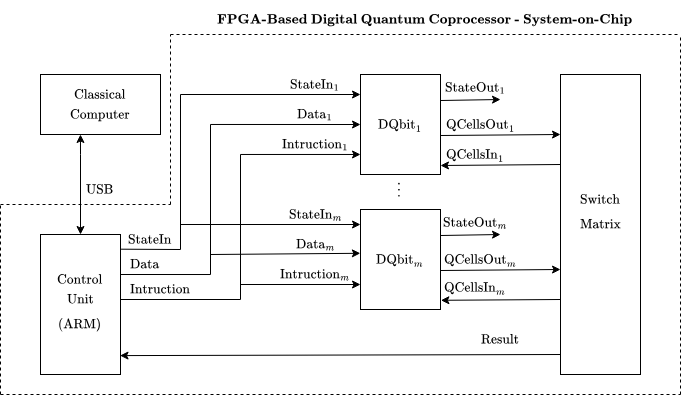
\includegraphics[width=1.0\linewidth]{body/ch3/figs/hlukhov-digital-qc}
	\caption[Generalised Functional Diagram of an Emulated Digital Quantum Computer by Hlukhov.]{A digital quantum computer consists of a control element for initialising quantum states (\texttt{StateIn}\_j corresponding to the digital qubit labelled \texttt{DQbit}\_j). The switching matrix connects qubits to each other and returns the results to the control unit on the FPGA.}
	\label{fig:hlukhov-digital-qc}
\end{figure}

Hlukhov also defined a \textit{digital qubit} as a qubit that can be represented as a discrete finite state machine resulting from a unique chain of quantum gates \cite{Hlukhov2021}. Hlukhov's study focused on implementing the FPGA-based digital quantum coprocessor consisting of 4 to 128 qubits capable of performing the QFT. Each digital qubit consisted of a $j$ series-connected digital quantum cells describing a single operation that transforms the state code \texttt{State} of the measured state $\ket{Q_{0j}}$ as shown in figure \ref{fig:hlukhov-qubit} \cite{Hlukhov2021}. The state of qubits was conditionally described as $\ket{x_mx_{m-1}...x_1x_0}$, where each $x_j$ corresponds to the neutral position of the state vector in the unit circle at an angle of $\theta$. The movement of this state vector in the unit circle corresponds to the behaviour of a single qubit with real amplitudes of the probabilistic quantum state \cite{Hlukhov2021}. Hlukhov chose the polar coordinate system to represent the position of the vector in contrast to the Cartesian coordinate system which requires two values for the input and the output \cite{Hlukhov2021}. 

\begin{figure}[!ht]
	\centering
	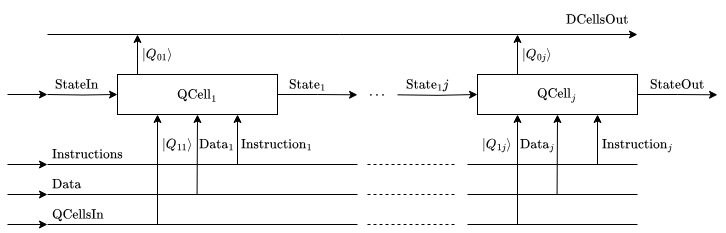
\includegraphics[width=1.0\linewidth]{body/ch3/figs/hlukhov-qubit}
	\caption[Digital Qubit (DQbit) by Hlukhov.]{Hlukhov's digital quantum qubit (DQbit) consists of quantum cells (QCell) that receive the initial state $StateIn$, instructions and data from the external control unit \cite{Hlukhov2021}.}
	\label{fig:hlukhov-qubit}
\end{figure}

The quantum cells were arranged such that the first cell in the series receives the initial state code from the external control unit and the last cell in the series stores the status code of the final qubit state in an output pipeline register \cite{Hlukhov2021}. Additionally, each quantum cell receives the measured state $\ket{Q_{1j}}$ of another qubit from the switch matrix \cite{Hlukhov2021}. The probabilistic nature of quantum measurements of qubits was enabled by a pseudo-random number generator in the measuring unit facilitated by the FPGA ROM \cite{Hlukhov2021}. 

The pseudo-random number generator produced values such that in the switch matrix, the probability of measuring input states in the computational basis with an odd parity of bits was equal to the probability of measuring state codes with even parity \cite{Hlukhov2021}. In other words, Hlukhov distributed the probability of measuring each state according to the parity of state code in the computational basis. The results from the experiment using digital qubits in this manner on the FPGA-based digital quantum coprocessor showed that the execution time of the QFT does not depend on the number of qubits in the coprocessor and is commensurate with the decoherence time of electron-spin-based qubits, i.e. about $\SI{10}{\nano\second}$ \cite{Hlukhov2021}. For instance, the results showed that the percentage of FPGA resources used when 10 qubits were emulated was $24\%$ and when 128 qubit digital quantum coprocessor was emulated, the resource usage percentage decreased to $14\%$ \cite{Hlukhov2021}.

In summary, careful consideration needs to be taken on the representation qubits as classical bits in the FPGA-based quantum computer emulation. The manner in which qubit quantum states are stored in memory is critical for the precision of the emulation. Furthermore, streamlining the definition of a quantum state is crucial for the performance of the design. Literature shows that the emulation time grows exponentially as the number of bits $n$ increases, however, when the representation of qubits is carefully selected, the percentage of FPGA resources that are used to emulate qubits can be independent of the number of qubits \cite{Hlukhov2021, hong2022quantum}. The following section provides a review on how quantum gates and quantum circuits are performed classically to emulate a quantum computing algorithms on a FPGA. 
%such as the Bell state given by 
%\begin{align}
%	\ket{\psi} & = \alpha_{00}\ket{00} + \alpha_{01}\ket{01} + \alpha_{10}\ket{10} + \alpha_{11}\ket{11}
%\$end{align}

\section{Emulating Quantum Gates and Quantum Circuits on FPGAs \label{sec:lit-fpga-qgate-qcircuit}}

FPGA architectures depend on the constraints of logic element structures, programmable interconnect structures, interconnection networks, configuration, and different types of wires, including local, global and general purpose wires \cite{wolf2004fpga}. Programmable logic blocks and programmable interconnects provide multi-level logic and parallelism which is suitable for the emulation of quantum gates and their effect on qubits in a quantum circuit. Efficient use of the resources on the FPGA can allow quantum algorithms to be emulated in a shorter time by sequence of quantum gate operations is performed appropriately based on the constraints of the device. The most commonly implemented is the QFT due to its applicability in various quantum algorithms as described in the theoretical framework in chapter \ref{ch:theoretical_framework}. 

\subsection{Implementing Gates to Solve a Problem Function}

Using the input-and-output table described in the previous section, Fujishima emulated the QFT to solve an NP-complete for periodic function $f(x)$ in polynomial time. In order to apply the QFT, the outputs of the table must be periodic, otherwise Grover's algorithm is used to search for a specific value from the table \cite{fujishima2003fpga}. To generate the table in polynomial time, Fujishima applied the \textit{satisfiability} problem which finds a group of variables that satisfy a given Boolean equation \cite{fujishima2003fpga}. Fujishima used the FPGA emulator to execute a satisfiability algorithm for the Boolean equation given by
\begin{align}
	(\bar{a}+c+\bar{d})\cdot(\bar{b}+\bar{e})\cdot(a+d+\bar{f}+h)\cdots(k+g)=1\nonumber
\end{align}
At the start of the emulation, the outputs corresponding to all variables were initialised to 0 by applying De Morgan's laws and negating both sides of the above satisfiability equation. The terms in the brackets of the equation were divided into nodes. In the final stage, binary search was used to investigate the input corresponding to the output with 0 to obtain the answer \cite{fujishima2003fpga}. 

\subsection{Emulating Quantum Gate Operations Using a Logic Cells}

Using a more conventional approach to emulating quantum operations on qubits, Khalid et al. developed a VHDL library of common quantum gates comprising of the Hadamard, \texttt{CNOT}, \texttt{X}, \texttt{Z} and phase shift gate \cite{Khalid2004}. In addition to using VHDL for mapping the quantum gates to code, Khalid et al. employed the code generating capabilities of VHDL to automatically produce descriptions of multiple input quantum gates from single-input gates \cite{Khalid2004}. This is in line with Barenco et al.'s observation that multi-qubit gates can be constructed using a series of single-qubit Pauli-gates and \texttt{CNOT} gates. Intuitively, single-qubit gates required less resources than the other gates. Controlled gates were initialised by passing the number of control variables as a parameter to the code generating script which produced the VHDL description of the resulting transformation \cite{Khalid2004}. This procedure allowed Khalid et al. to automate the construction of arbitrary size quantum gates using clock synchronised quantum state registers (QSR) that can represent the state of the quantum system at any given stage in the flow of data \cite{Khalid2004}. Gates that produce entangled states required considerably more resources than gates where no entanglement occurred due to \cite{Khalid2004}. Figure \ref{fig:khalid-q-evo} illustrates the emulation of quantum evolution of an entangled system for the case of two qubits $\psi_1$ and $\psi_2$ that are used as the control and target qubit of the \texttt{CNOT} gate. In this case, the \texttt{CNOT} gate requires 4 complex multiplications \cite{Khalid2004}. In general, a $n$ input \texttt{CNOT} gate requires $2^n$ complex multiplications \cite{Khalid2004}. Khalid et al. noted that this exponential increase in resource requirement for emulating entanglement poses a fundamental bottleneck in modelling quantum systems by classical means \cite{Khalid2004}. 

\begin{figure}[!ht]
	\centering
	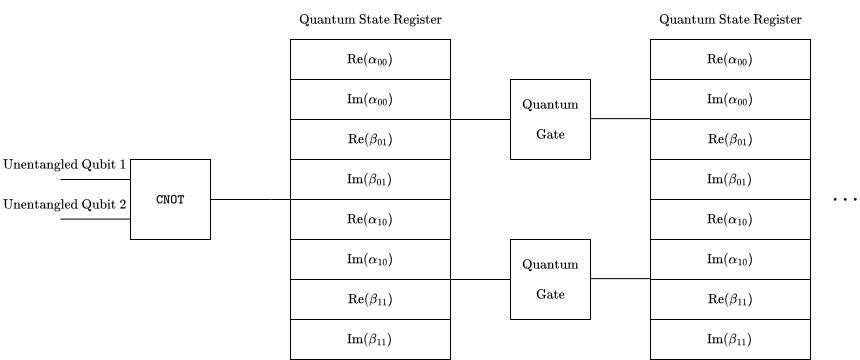
\includegraphics[width=1.0\linewidth]{body/ch3/figs/khalid-q-evo}
	\caption[Showing Use of Quantum Registers in a Quantum Circuit Evolution by Khalid et al.]{Quantum state registers represent the state of the entire system at a given stage in the evolution of a quantum circuit \cite{Khalid2004}.}
	\label{fig:khalid-q-evo}
\end{figure}

Khalid et al. successfully used logic cells for quantum gates in the VHDL library to emulate the quantum circuits associated with the QFT and Grover's search algorithm for a 4 element database using 3-qubits \cite{Khalid2004}. The most commonly used quantum gate was the Hadamard gate. In the case where 16-bit mantissas were used to achieve a higher emulation accuracy, 1284 logic cells were used to emulate Hadamard gate operations on an Altera Stratix FPGA \cite{Khalid2004}. About 580 less logic cells were required to achieve a lower emulation accuracy using 8-bit mantissas for the same operations using the Hadamard gate \cite{Khalid2004}. Khalid et al. highlighted that since $X$ and $Z$ gates do not use logic cells because the swap and bit flip operations performed consume negligible resources \cite{Khalid2004}. The same clock speed of $\SI{82.1}{\mega\hertz}$ was used to emulate the QFT and Grover's search algorithm using the logic cell quantum gates. However, Grover's search algorithm used more logic cells in total. While emulating the 3-qubit QFT with 16-bit mantissas used 5076 logic cells in total, emulating Grover's search algorithm consumed 12636 logic cells. 

\subsection{Emulating Quantum Gates that Produce Entangled States}

The proposed method by Aminian et al., which employed fixed-point numbers to represent the normalised coefficients as described in the previous section, also implemented the $X$, $Z$, \texttt{CNOT}, phase shift and Hadamard gate. However, the main difference between Khalid et al. and Aminian et al.'s implementation of these universal quantum gates is that instead of using QSRs to represent the stage of evolution of the quantum states, Aminian et al.'s FPGA emulated Pauli and controlled gates were implemented using three additional bits labelled $b$, $i$, and $s$, corresponding to the basis, complexity and sign \cite{Aminian2008}. To emulate Pauli gate operations, the bits were manipulated as illustrated in figure \ref{fig:aminian-pauli-gates}. Similar to Khalid et al.'s implementation, Aminian et al.'s design required more computational resources for emulating quantum entanglement \cite{Aminian2008, Khalid2004}. For example, applying the single-qubit Hadamard gate on a single qubit required four multipliers and four adders, while applying the same gate on three entangled qubits $\ket{j_1 j_2 j_3}$ required sixteen multipliers and sixteen adders \cite{Aminian2008}. 
\begin{figure}[!ht]
	\centering
	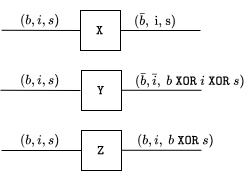
\includegraphics[width=0.75\linewidth]{body/ch3/figs/aminian-pauli-gates}
	\caption[Implementation of Paul-$X$, $Y$, and $Z$ Gates by Aminian et al.]{Using the bits to represent the basis ($b$), the complexity ($i$) and sign ($s$), Aminian et al. were able to implement the single-qubit Pauli gates showing above \cite{Aminian2008}.}
	\label{fig:aminian-pauli-gates}
\end{figure}

To emulate the \texttt{CNOT} gate, additional qubits were appended to the entangled bit $b$ in the computation basis. Hadamard and controlled-$R$ gates, were implemented in a similar manner to Khalid et al.'s implementation where intermediate QSRs are used to keep track of the quantum states of the quantum computer \cite{Aminian2008, Khalid2004}. When both groups of gates were used, the gate operations were implemented by a coefficient swapping operator \cite{Aminian2008}. In this case, the $X$ gate was implemented with four registers and the $Z$ gate was implemented by multiplying the $\beta$-coefficient of the quantum state by -1 \cite{Aminian2008}. Aminian et al. designed the emulation method using VHDL and evaluated various library gates in both distinct and entangled 3-qubit states for performing the QFT and Grover's search algorithm \cite{Aminian2008}. Aminian et al.'s method used significantly less logic cells on the Altera Stratix FPGA compared to Khalid et al.'s implementation on the same board. For example, when using 16-bit mantissas to perform the QFT, Khalid et al.'s implementation required only 8197 logic cells compared to the 12636 logic cells required in Khalid et al.'s emulator \cite{Aminian2008, Khalid2004}. However, Aminian et al.'s synchronised each block of the emulation stage using a higher clock frequency of $\SI{131.3}{\mega\hertz}$ \cite{Aminian2008}. 

\subsection{Adjusting State Machine Corresponding to Unitary Operations}

Mohamed et al.'s implementation of two angles from the spherical coordinates of the quantum state of qubits used a state machine in VHDL to calculate the matrix tensor products in the Deutsch-Jozsa algorithm. The size of the matrix tensor products was determined by the total number of qubits in the quantum computer \cite{mohamed2009using}. VHDL blocks adjusted the state machine in order to produce the tensor product operation matrix associated with 3 Hadamard gates and one \texttt{CNOT} gate. The overall design flow proposed by Mohamed et al. for hardware acceleration using an FPGA are shown in figure \ref{fig:mohamed-design-flow} where the VHDL generation step refers to connecting the chain of operations after setting up the generic parameters which define the number of qubits and the number of operations \cite{mohamed2009using}. 

%TODO
%Mohamed-design-flow


\subsection{Quantum Fourier Transform Implementations using DSP Blocks}

Rivera-Miranda, Caicedo-Beltr\'{a}n, Valencia-Pay\'{a}n, Espino-Duran, and Velasco-Medina addressed the shortcomings of software simulators by presenting a hardware design of an emulator for computing the QFT using FPGAs in 2011 \cite{rivera2011hardware}. The proposed hardware design methodology differs from the ones by Fujishima, Khalid et al., Aminian et al. and Mohamed et al. in that it used a fixed-point two's complement representation with 2 bits in the integer part. Instead of matrix operations which would require a lot of hardware resources, Rivera-Miranda et al. designed quantum gates using building blocks, with sum, subtract or multiply only when it is necessary \cite{rivera2011hardware}. For example, similar to the implementation by Aminian et al., the Hadamard gate used four multipliers and four adders, whereas the controlled phase shift or controlled-$R$ gate required four multipliers and two adders as illustrated in the block diagrams in figure \ref{fig:rivera-hadamard-gate} \cite{rivera2011hardware}. This architecture of these quantum gate emulations was described in VHDL where the user parameters were the number of qubits, the number of mantissa bits and the pipeline depth \cite{rivera2011hardware}. 

The operation of the circuit was successfully verified over two clock cycles using ModelSim-Altera to simulate a 4-qubit quantum computer using a 16-bit mantissa to improve computational accuracy \cite{rivera2011hardware}. On the first cycle of the simulation, the given input state, \textit{iqubit} was $\ket{j} = \ket{0111}$ and on the second cycle, the output signal \textit{oqubit} was the quantum state $\ket{y} = \ket{y_1 y_2 y_3 y_4}$, where
\begin{align}
	y_1	 & = 0.7071\ket{0} - 0.7071\ket{1}\nonumber\\
	y_2	 & = 0.7071\ket{0} - j0.7071\ket{1}\nonumber\\
	y_3	 & = 0.7071\ket{0} + (-0.5000 + j0.5000)\ket{1}\nonumber\\
	y_4	 & = 0.7071\ket{0} + (-0.2706 + j0.6533)\ket{1}\nonumber
\end{align}
which corresponds to the expected transformation at the end of the QFT quantum circuit \cite{rivera2011hardware}. Rivera-Miranda were able to synthesise the design on the Altera Stratic FPGA as depicted in the block diagram in figure \ref{fig:rivera-block-diagram} using the Quartus II Professional software suite \cite{rivera2011hardware}. The diagram includes a multiplexer at the parallel output which was used to present the resulting qubits one-by-one once all the input qubits had been loaded and after a number of cycles given by the latency \cite{rivera2011hardware}. 

%TODO
%Rivera 

Another difference in Rivera-Miranda's implementation is that the QFT was implemented using Altera's IP cores that use mainly 18-bit DSP blocks and the distributed memory bits to reduce the number of hardware resource required \cite{rivera2011hardware}. Results from the synthesis of the QFT on FPGA were summarised into the number of adaptive LUTs, registers and DSP blocks. These results showed a linear increase in the number adaptive LUTs and registers while there were available DSP blocks, and an exponential increase when there were not available DSP blocks \cite{rivera2011hardware}. To emulate 16-qubits, 14786 adaptive LUTs, 3537 logic registers, 768 9-bit DSP blocks were employed at a maximum clock frequency of $\SI{83.10}{\mega\hertz}$ \cite{rivera2011hardware}. The clock frequency decreased as the number of qubits in the emulated quantum computer increased.

\subsection{Concurrent vs Sequential Implementations of Quantum Gate Operations}

More recently in 2014, Lee, Khalil-Hani and Marsono conducted experiments based on the QFT to identify suitable qubit representation and hardware design techniques for manage resources that grow exponentially as the number of qubits in the system grows \cite{lee2014fpga}. Lee et al. suggested that the QFT is a suitable candidate as an entry-level case study for quantum circuit emulation because it can be easily mapped into a simple quantum circuit \cite{lee2014fpga}. Furthermore, Lee et al. distinguished between concurrent, pipelined, and serial processing for emulating quantum circuit classically. Concurrent processing allows parallelism which completes all computations within on clock cycle while pipeline processing includes additional registers as illustrated in figure \ref{fig:lee-concurrent-v-pipeline} \cite{lee2014fpga}.

\begin{figure}[!ht]
	\centering
	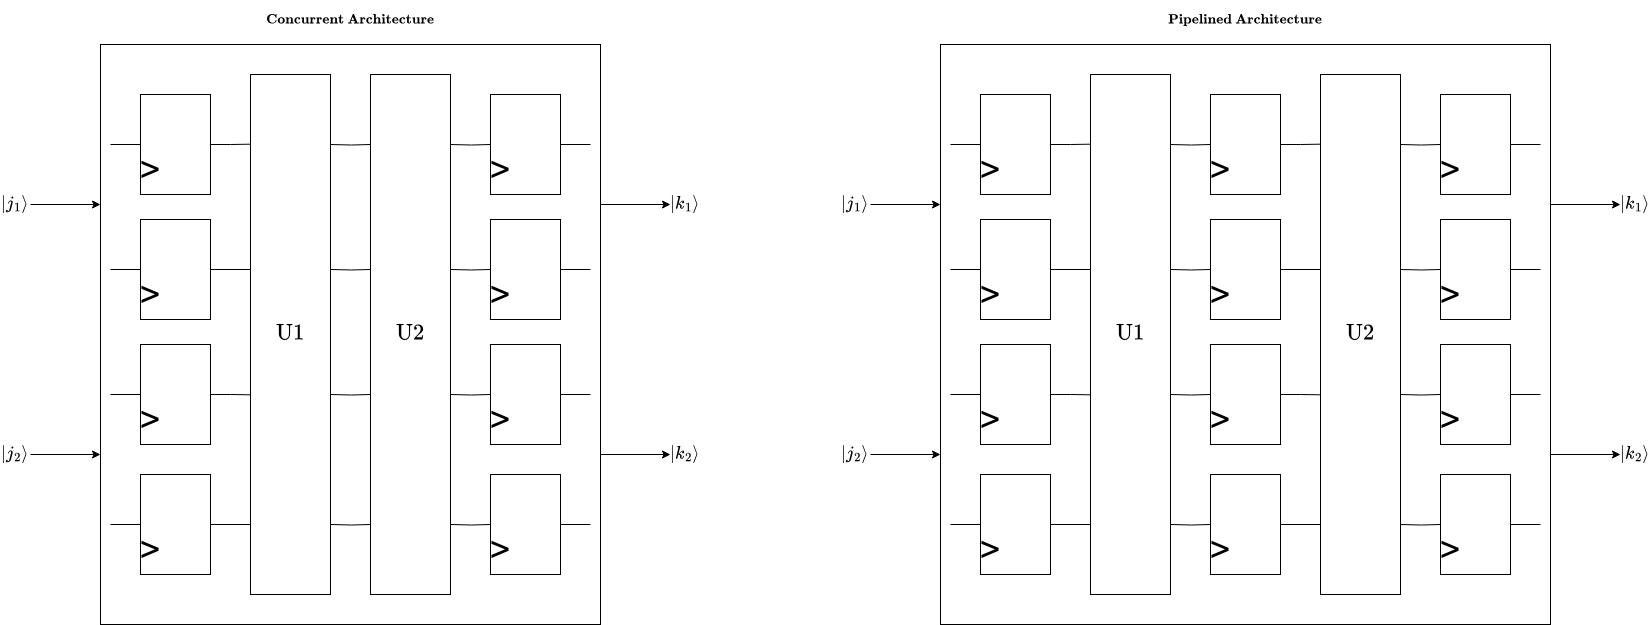
\includegraphics[width=1.0\linewidth]{body/ch3/figs/lee-concurrent-vs-pipeline}
	\caption[Side-by-Side Comparison of Concurrent and Pipelined Emulation by Lee et al.]{Concurrent emulation (left) allows for parallelism in that all the quantum gate operations are performed before the output states are produced. A pipelined design (right) is more suitable for producing high throughput with low critical path delays due to the insertion of registers after each stage of the unitary transformation \cite{lee2014fpga}.}
	\label{fig:lee-concurrent-v-pipeline}
\end{figure}

Although a concurrent technique can allow parallelism and effective resource management, Lee et al. noted that this would lead to a high critical path delay and low operating frequency \cite{lee2014fpga}. The advantage of using a serial architecture is that it increases throughput and decreases the critical path delay while presenting the designer with the opportunity to utilise resource sharing through shared registers as illustrated in figure \ref{fig:lee-serial-architecture} \cite{lee2014fpga}. The results also showed that a serial design achieves balance on both resource utilisation and operating frequency as the number of dedicated logic registers in the serial architecture was reduced for a constant operating frequency \cite{lee2014fpga}. Additionally, the experiments showed that a 16-bit fixed-point representation introduced significant precision error for both 2-qubit and 5-qubit QFT emulations \cite{lee2014fpga}. The precision error of the 2-qubit QFT was successfully reduced to zero by expanding the number of mantissa bits up to 22 bits, or a total of 24 bits \cite{lee2014fpga}.

\begin{figure}[!ht]
	\centering
	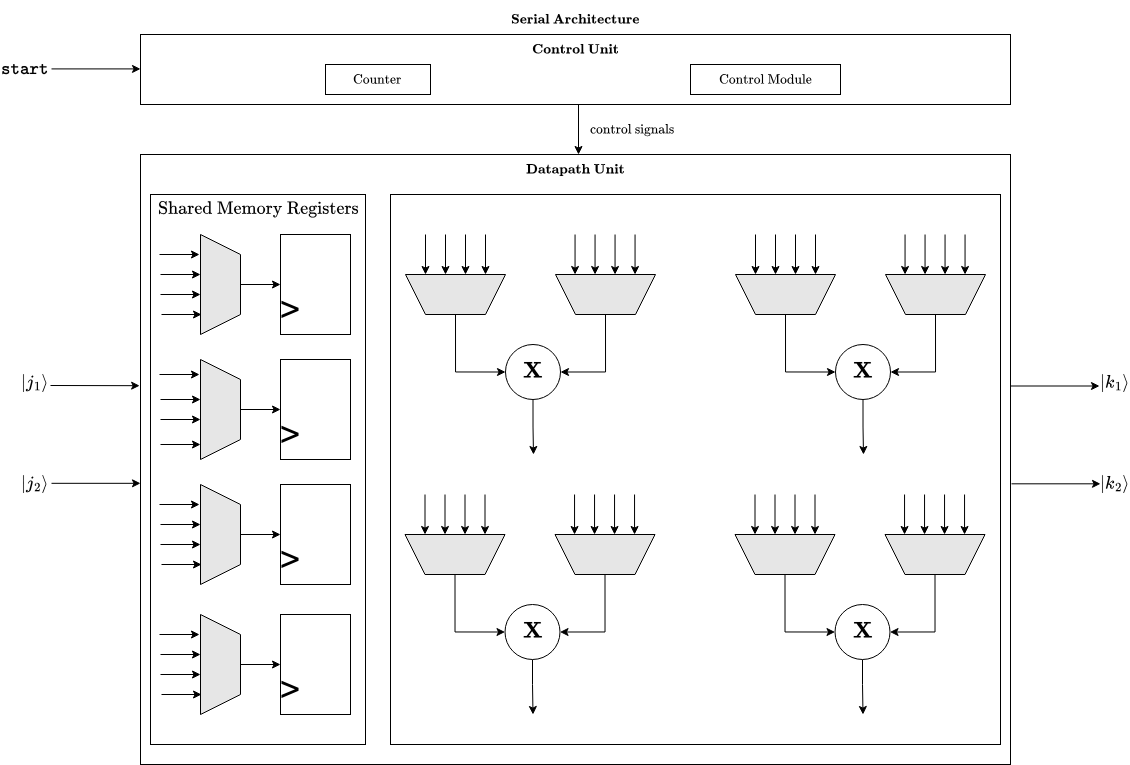
\includegraphics[width=1.0\linewidth]{body/ch3/figs/lee-serial-architecture}
	\caption[Serial Architecture of Emulated Quantum Computer by Lee et al.]{The following diagram illustrates the serial architecture for a 2-qubit quantum computer emulator. Although the serial architecture may require more iterations than the concurrent and pipelined architectures, it offers resource sharing which can be considerably beneficial in terms of resource management \cite{lee2014fpga}s. Here, the multiplication symbols illustrate the product of the inputs with the probabilistic coefficients.}
	\label{fig:lee-serial-architecture}
\end{figure}

However, the short-coming of this implementation is that it does not consider the coupling of qubits, as required by DiVincenzo's criterion regarding well-characterised qubits. 

\subsection{Emulated Quantum Gate }
 
The study focused on implementing the digital quantum coprocessor on FPGA to factorise the integer $(15)_{10}$ using Shor's algorithm. To emulate quantum gates in the FPGA-based digital quantum computer, Hlukhov began by distinguishing between a quantum gate in an analog quantum computer and a digital quantum gate in a digital quantum computer \cite{hlukhov}. Hlukhov took a quantum gate in an analog quantum computer to only symbolise the operation of changing the position of a vector on a Bloch sphere or in a unit circle \cite{Hlukhov2021}. In contrast, a digital quantum gate in a digital quantum computer was taken to represent a digital device that changes the internal code of a qubit as a finite state machine, corresponding to a change in the intermediate position of a single vector on a Bloch sphere or in a unit circle \cite{Hlukhov2021}. Similar to previous implementations that used pipeline QSRs, Hlukhov introduced a model of digital quantum gate that includes an ALU, a comparator and a pipeline register as seen in figure \ref{fig:hlukhov-qgate} \cite{Hlukhov2021}. 

\begin{figure}[!ht]
	\centering
	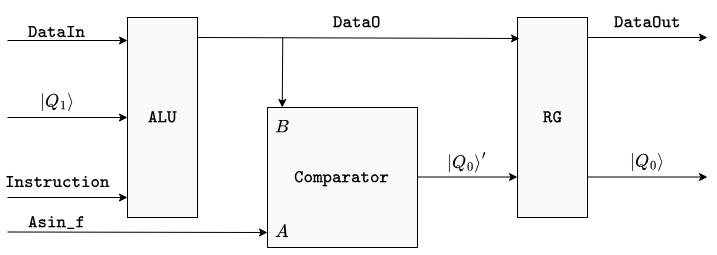
\includegraphics[width=1.0\linewidth]{body/ch3/figs/hlukhov-qgate}
	\caption[Proposed Quantum Gate by Hlukhov.]{Model of a digital quantum gate that includes an ALU, a comparator and a pipeline.}
	\label{fig:hlukhov-qgate}
\end{figure}

In the digital quantum gate model, the output of the gate is represented by the qubit state code \texttt{DataOut} and the measured state $\ket{Q_0}$ of a qubit is taken from the pipeline register \cite{Hlukhov2021}. An intermediate status code, \texttt{DataO}, is evaluated in the comparator with the random variable \texttt{Asin\_f} to obtain the measured state $\ket{Q_0}'$. The only types of quantum gates that were emulated using this implementation were the Hadamard and the controlled phase shift gates. After performing the QFT, the expected output was $80000000_{16}$, corresponding to the number of periods \cite{Hlukhov2021}. It was shown that the probability of obtaining true results increases rapidly with a decrease in the state code length \cite{hlukhov2021digital}. 

\subsection{Memory Considerations for Emulating Quantum Gates}

In 2022, Hong, Jeon and Park proposed a hardware architecture which operates based on a single-input gate regardless of the number of qubits used in the circuit \cite{hong2022quantum}. The proposed architecture was implemented on a FPGA using an Advanced Peripheral Bus (APB) interface for setting parameters such as gate data and an Advanced High-performance Bus (AHB) interface for communication with external memory \cite{hong2022quantum}. The aim of the implementation was to reduce unnecessary multiplications and data transfer with SDRAM external memory \cite{hong2022quantum}. The QFT quantum circuit was emulated in three stages, with each gate performed in the circuit one by one. 

In the first stage, state grouping was performed using the characteristic that an element of the output state vector, which applied by a single-qubit gate, is only affected by two elements of the input state vector \cite{hong2022quantum}. Since a single-qubit gate is only applied to one qubit, it cannot modify the state of the other qubit in the group. At the end of the state grouping stage, pairs of states were sent to the second stage where unnecessary data transfer from external memory was eliminated \cite{hong2022quantum}. This is performed by skipping data transfer if an element of the output state does not change from that of the input state \cite{hong2022quantum}. Furthermore, control-gates were skipped when the control-bit was 0 since states are only transformed when the control qubit is 1 \cite{hong2022quantum}. Hong et al. reported that using this scheme, half of the output states can be skipped to reduce multiplication operations and data transfer from external memory \cite{hong}. In the final stage of the finite state machine describing the implementation, matrix elements of the input state vector were multiplied by the $2\times2$ unitary matrix of the quantum gate. The output state was produced using the grouped states from the first stage. 

Hong et al.'s architecture was synthesised and emulated on a Xilinx Kintex UltraScale (XCKU115) FPGA platform at $\SI{160}{\mega\hertz}$. The implementation used 19204 LUTs, 4027 registers and 128 DSP blocks \cite{hong2022quantum}. In addition, the architecture used a 16-bit fixed point precision for representing data, equating to a total of 32 bits used for storing a single complex number corresponding to a state vector \cite{hong2022quantum}. Experimental results showed that emulation time grew exponentially as the number $n$ of qubits increased, according to the dimensions of the quantum state vector \cite{hong2022quantum}. 

\section{Testing and Benchmarking the Performance of FPGA-Based Quantum Computer Emulators}

In most of the literature explored above where quantum computers have been emulated on FPGAs, the design is evaluated by comparing resource usage and execution times with previous implementations. For example, Aminian et al. use the results from Khalid et al.'s implementation to compare the total number of logic cells required by the design \cite{Aminian2008, Khalid2004}. As quantum computing operations involve dense matrices, careful consideration must be taken regarding testing and benchmarking the performance of the FPGA design. 

In 2024, Lee Belfore II proposed a scalable accelerator architecture specifically to solve the challenge of managing parallelism by efficiently routing quantum state components for gate evaluation and measurement \cite{belfore2024scalable}. Belfore demonstrated the architecture on an Intel Agilex AGFB014 FPGA on the Intel Agilex F-series FPGA development kit using a fixed-point scheme. Belfore noted that in order to support high performance data processing, DSPs can provide optimised and flexible multipliers, adders, and registers that facilitate high speed operation and efficient pipeline \cite{belfore2024scalable}. Subsequently, memory in the vicinity of DSP blocks reduce latencies incurred by sourcing operands. Belfore identified the usefulness of ARM based processor cores, that many FPGAs offer, in coordinating high level operation and tasking \cite{belfore2024scalable}. 

According to Belfore, since algorithms on FPGAs can be implemented by mapping an algorithm to a state machine this implemented directly on the FPGA, the state machines can be organised heirarchically in order to manage high level states related to phases of the computation and low level state machines that are synchronised on a clock cycle \cite{belfore2024scalable}. State machines can be implemented using Verilog which can simulate the evolution of qubits in a quantum circuit using a testbench. In their study, Belfore implemented the quantum emulator at the RTL level using the IEEE 2008 standard release of VHDL. A simple circuit consisting of a layer of Hadamard gates was simulated using the open-source VHDL platform GHDL \cite{belfore2024scalable}. 

Belfore used permutations of the inputs to align quantum state register elements to functional units on the FPGA \cite{belfore2024scalable}. Furthermore, Belfore stated that accessing the state vector in the quantum state register needs to be conducted linearly on a classical computer, therefore retrieving and operating on any component requires $\mathcal{O}(2^n)$ time \cite{belfore2024scalable}. One of the suggested improvements to the slow read and write operations is to use non-blocking permutation networks which require $\mathcal{O}(\log n)$ switching layers \cite{belfore2024scalable}.

The operation of the quantum emulator was verified by comparing results with the QuEST quantum computing simulation platform \cite{belfore2024scalable}. Belfore found that the standard deviation between the empirically derived probability distributions was $1.21\times10^{-4}$, and a mean absolute error of $1.36\times10^5$, which suggested a good agreement between the FPGA-based quantum emulator and the QuEST simulator \cite{belfore2024scalable}. Additionally, Belfore evaluated the performance of the FPGA emulator by reporting the required clocks per individual circuit emulation, clock period, and the time required for an individual emulation \cite{belfore2024scalable}. In total, results showed that the emulation time on the Intel Agilex FPGA was $\SI{14}{\micro\second}$, while the random circuit simulation using QuEST on a XEON ES-2603 v2 $\SI{1.8}{\giga\hertz}$ processor required $\SI{5.25}{\milli\second}$ of CPU time - equating to a performance speedup of 368 using the FPGA \cite{belfore2024scalable}.
